% Template for PLoS
% Version 3.4 January 2017
%
% % % % % % % % % % % % % % % % % % % % % %
%
% -- IMPORTANT NOTE
%
% This template contains comments intended 
% to minimize problems and delays during our production 
% process. Please follow the template instructions
% whenever possible.
%
% % % % % % % % % % % % % % % % % % % % % % % 
%
% Once your paper is accepted for publication, 
% PLEASE REMOVE ALL TRACKED CHANGES in this file 
% and leave only the final text of your manuscript. 
% PLOS recommends the use of latexdiff to track changes during review, as this will help to maintain a clean tex file.
% Visit https://www.ctan.org/pkg/latexdiff?lang=en for info or contact us at latex@plos.org.
%
%
% There are no restrictions on package use within the LaTeX files except that 
% no packages listed in the template may be deleted.
%
% Please do not include colors or graphics in the text.
%
% The manuscript LaTeX source should be contained within a single file (do not use \input, \externaldocument, or similar commands).
%
% % % % % % % % % % % % % % % % % % % % % % %
%
% -- FIGURES AND TABLES
%
% Please include tables/figure captions directly after the paragraph where they are first cited in the text.
%
% DO NOT INCLUDE GRAPHICS IN YOUR MANUSCRIPT
% - Figures should be uploaded separately from your manuscript file. 
% - Figures generated using LaTeX should be extracted and removed from the PDF before submission. 
% - Figures containing multiple panels/subfigures must be combined into one image file before submission.
% For figure citations, please use "Fig" instead of "Figure".
% See http://journals.plos.org/plosone/s/figures for PLOS figure guidelines.
%
% Tables should be cell-based and may not contain:
% - spacing/line breaks within cells to alter layout or alignment
% - do not nest tabular environments (no tabular environments within tabular environments)
% - no graphics or colored text (cell background color/shading OK)
% See http://journals.plos.org/plosone/s/tables for table guidelines.
%
% For tables that exceed the width of the text column, use the adjustwidth environment as illustrated in the example table in text below.
%
% % % % % % % % % % % % % % % % % % % % % % % %
%
% -- EQUATIONS, MATH SYMBOLS, SUBSCRIPTS, AND SUPERSCRIPTS
%
% IMPORTANT
% Below are a few tips to help format your equations and other special characters according to our specifications. For more tips to help reduce the possibility of formatting errors during conversion, please see our LaTeX guidelines at http://journals.plos.org/plosone/s/latex
%
% For inline equations, please be sure to include all portions of an equation in the math environment.  For example, x$^2$ is incorrect; this should be formatted as $x^2$ (or $\mathrm{x}^2$ if the romanized font is desired).
%
% Do not include text that is not math in the math environment. For example, CO2 should be written as CO\textsubscript{2} instead of CO$_2$.
%
% Please add line breaks to long display equations when possible in order to fit size of the column. 
%
% For inline equations, please do not include punctuation (commas, etc) within the math environment unless this is part of the equation.
%
% When adding superscript or subscripts outside of brackets/braces, please group using {}.  For example, change "[U(D,E,\gamma)]^2" to "{[U(D,E,\gamma)]}^2". 
%
% Do not use \cal for caligraphic font.  Instead, use \mathcal{}
%
% % % % % % % % % % % % % % % % % % % % % % % % 
%
% Please contact latex@plos.org with any questions.
%
% % % % % % % % % % % % % % % % % % % % % % % %

\documentclass[10pt,letterpaper]{article}
\usepackage[top=0.85in,left=2.75in,footskip=0.75in]{geometry}

% amsmath and amssymb packages, useful for mathematical formulas and symbols
\usepackage{amsmath,amssymb}

% proper font greek letters
\usepackage{upgreek}

% Tabu environment
\usepackage{tabu}

% Reference sections by name
\usepackage{nameref}

% Maximum fraction of the page height a figure may take and still allow text to float below it.
%\renewcommand{\floatpagefraction}{.8}
\renewcommand{\topfraction}{.95}

% Use adjustwidth environment to exceed column width (see example table in text)
\usepackage{changepage}

% Use Unicode characters when possible
\usepackage[utf8x]{inputenc}

% textcomp package and marvosym package for additional characters
\usepackage{textcomp,marvosym}

% cite package, to clean up citations in the main text. Do not remove.
\usepackage{cite}

% Use nameref to cite supporting information files (see Supporting Information section for more info)
\usepackage{nameref,hyperref}

% line numbers
\usepackage[right]{lineno}

% ligatures disabled
\usepackage{microtype}
\DisableLigatures[f]{encoding = *, family = * }

% color can be used to apply background shading to table cells only
\usepackage[table]{xcolor}

% array package and thick rules for tables
\usepackage{array}

% create "+" rule type for thick vertical lines
\newcolumntype{+}{!{\vrule width 2pt}}

% create \thickcline for thick horizontal lines of variable length
\newlength\savedwidth
\newcommand\thickcline[1]{%
  \noalign{\global\savedwidth\arrayrulewidth\global\arrayrulewidth 2pt}%
  \cline{#1}%
  \noalign{\vskip\arrayrulewidth}%
  \noalign{\global\arrayrulewidth\savedwidth}%
}

% \thickhline command for thick horizontal lines that span the table
\newcommand\thickhline{\noalign{\global\savedwidth\arrayrulewidth\global\arrayrulewidth 2pt}%
\hline
\noalign{\global\arrayrulewidth\savedwidth}}


% Remove comment for double spacing
%\usepackage{setspace} 
%\doublespacing

% Text layout
\raggedright
\setlength{\parindent}{0.5cm}
\textwidth 5.25in 
\textheight 8.75in

% Bold the 'Figure #' in the caption and separate it from the title/caption with a period
% Captions will be left justified
\usepackage[aboveskip=1pt,labelfont=bf,labelsep=period,justification=raggedright,singlelinecheck=off]{caption}
\renewcommand{\figurename}{Fig}

% Use the PLoS provided BiBTeX style
\bibliographystyle{plos2015}

% Remove brackets from numbering in List of References
\makeatletter
\renewcommand{\@biblabel}[1]{\quad#1.}
\makeatother

% Leave date blank
\date{}

% Header and Footer with logo
\usepackage{lastpage,fancyhdr,graphicx}
\usepackage{epstopdf}
\pagestyle{myheadings}
\pagestyle{fancy}
\fancyhf{}
\setlength{\headheight}{27.023pt}
\lhead{
\includegraphics[width=2.0in]{PLOS-submission.eps}}
\rfoot{\thepage/\pageref{LastPage}}
\renewcommand{\footrule}{\hrule height 2pt \vspace{2mm}}
\fancyheadoffset[L]{2.25in}
\fancyfootoffset[L]{2.25in}
\lfoot{\sf PLOS}

%% Include all macros below

\newcommand{\lorem}{{\bf LOREM}}
\newcommand{\ipsum}{{\bf IPSUM}}

%% END MACROS SECTION


\begin{document}
\vspace*{0.2in}

% Title must be 250 characters or less.
\begin{flushleft}
{\Large
\textbf\newline{
Diffusive homeostasis in a self-organizing recurrent neural network: local neuron density predicts firing rates
} % Please use "sentence case" for title and headings (capitalize only the first word in a title (or heading), the first word in a subtitle (or subheading), and any proper nouns).
}
\newline
% Insert author names, affiliations and corresponding author email (do not include titles, positions, or degrees).
\\
Fabian Schubert\textsuperscript{1,2\Yinyang *},
Daniel Miner\textsuperscript{1,3\ddag},
Jochen Triesch\textsuperscript{1\dag},
\\
\bigskip
\textbf{1} Frankfurt Institute for Advanced Studies, Frankfurt am Main, Germany

\textbf{2} Goethe University Frankfurt, Institute for Theoretical Physics, Frankfurt am Main, Germany

\textbf{3} University of Göttingen, Third Institute of Physics, Göttingen, Germany
\\
\bigskip

% Insert additional author notes using the symbols described below. Insert symbol callouts after author names as necessary.
% 
% Remove or comment out the author notes below if they aren't used.
%
% Primary Equal Contribution Note
\Yinyang This author performed parts of the programming, analysis and writing and contributed to the conceptualization. Most of the author's work was carried out as a member of \textbf{1}.\\
% Additional Equal Contribution Note
% Also use this double-dagger symbol for special authorship notes, such as senior authorship.
\ddag This author performed parts of the programming, provided significant expertise and consultation and contributed to the conceptualization. Most of the author's work was carried out as a member of \textbf{1}.\\

\dag This author provided significant expertise and consultation and contributed to the conceptualization.

% Use the asterisk to denote corresponding authorship and provide email address in note below.
* E-mail: fschubert@fias.uni-frankfurt.de

\end{flushleft}
% Please keep the abstract below 300 words
\section*{Abstract}
%The topology of cortical networks is subject to constant change and the mechanisms involved in these dynamics are strongly influenced by the timing and intensity of neural spiking within these networks. Consequently, the success of a realistic biologically based computational model of synaptic structure and self-organization largely depends on an accurate modeling of neural activity. Experiments have found evidence for a broad, log-normal distribution of firing rates among cortical neurons.
%It is suggested that this heterogeneity of cortical activity has a functional role in the context of stimulus encoding and the formation of stable subpopulations of synapses.

%Building upon on a self-organizing spiking neural network (LIF-SORN), we replaced an intrinsic homeostatic control system used in earlier versions by a mechanism based on the diffusion of a neurotransmitter across the nervous tissue. The model of diffusive homeostasis was adopted from a previously published theoretical study. The main goal of this modification was to allow for the aforementioned broad and heavy tailed distribution of firing rates among the excitatory neural population, which could not be achieved by the formerly used single-cell homeostatic mechanism, binding firing rates of all neurons to a fixed target value. The resulting statistical features of spiking activity were positive regarding the desired firing rate statistics. Furthermore, we compared both homeostatic mechanisms with respect to features of synaptic network structures emerging throughout the simulation. Apart from the preservation of earlier reported non-random topological features, we found that diffusive homeostasis allowed for the emergence of neurons with strong outgoing synaptic efficacies. We could relate this feature of synaptic topology to the imposed spatial structure of the neural population by means of an analytic approach to the diffusive homeostatic steady state.
%% NEW VERSION
%The topology of cortical networks is subject to to constant change and the mechanisms involved in these dynamics are driven by the timing of neuronal spiking. Consequently, the success of a computational model of the self-organization of synaptic connectivity not only depends on the physiological accuracy of the plasticity mechanisms itself, but also on a realistic modeling of neuronal activity, e.g. since exact spike timing contains information on causal relations between pre- and postsynaptic activity. Experiments have found evidence for a strong heterogeneity among the average firing rates of cortical neurons, approximately following a log-normal distribution. In the context of synaptic plasticity it has been suggested that this property of neuronal firing has functional role in the formation of stable subnetworks. Furthermore, log-normal distributions are also known to well describe the statistics of synaptic efficacies in cortical networks. 
%
%We here present a self-organizing recurrent spiking network that exhibits log-normal statistics among the distribution of both synaptic weights, as well as of neuronal firing rates. To our knowledge, it is the first model that achieves this by means of a set of basic biologically motivated mechanisms, without the need for modifications that target specific experimental findings. Our model also comprises other features of synaptic connectivity that have been reported in experimental studies, such as an over representation of bidirectional connectivity.
%
%The presented network model is a combination of a self-organizing spiking neural network (LIF-SORN) and a recently proposed mechanism known as diffusive homeostasis, which has been shown to allow for a heavy-tailed, log-normal distribution of firing rates. Further investigating this concept, we found that the spatial configuration of neurons could determine individual homeostatic targets of activity in our network model, raising the question whether this effect might play a role in real cortical networks.
%NEW_NEW_VERSION
Firing rates of cortical neurons are very heterogeneous, approximately following a log-normal distribution. A similar log-normal like distribution also describes the efficacies of synapses connecting these neurons. Additionally, there is experimental evidence for an over-representation of bidirectional synaptic connectivity and power-law life-times of newly created synapses. It is presently unclear how all these features of cortical activity and wiring come about. Here we present a new spiking neural network model to explain these findings. The model is a member of the family of self-organizing recurrent neural network models with leaky integrate-and-fire neurons (LIF-SORN) and explains the above phenomena through the interaction of different plasticity mechanisms shaping network structure and dynamics. In particular, it incorporates a recently proposed mechanism for firing rate homeostasis based on the diffusion of nitric oxide. This mechanism supports a heavy-tailed, log-normal like distribution of firing rates. Interestingly, we find that the spatial configuration of neurons in the model determines individual homeostatic firing rate targets in the network. To understand this effect, we develop a theory to analytically describe the relationship between firing rates and local neuron density. The theory predicts that high firing rates are associated with low neuron density.
\newpage

% Please keep the Author Summary between 150 and 200 words
% Use first person. PLOS ONE authors please skip this step. 
% Author Summary not valid for PLOS ONE submissions.   
\section*{Author summary}
%We improved a model of self-organizing cortical network by implementing a model known as \textit{diffusive homeostasis}, which is capable of controlling neuronal activity based on the diffusion of a neurotransmitter. Previously reported non-random features of the network structure were preserved while allowing for a broader distribution of neuronal firing rates. Our modifications also led to the accumulation of strong synapses to a small subgroup of highly active neurons. By further analyzing the diffusive control, we found that the statistics of firing rates within the network are strongly affected by the structure of the neurons' positions. This raised the question whether the spatial structure of a cortical network, in particular fluctuations of neuronal densities, can influence activity not only by means of distance-dependent synaptic connection probabilities, but also through diffusive interaction.  
%% NEW VERSION
%Using a combination of a self-organizing recurrent network model and a mechanism known as diffusive homeostasis, we could reproduce experimental findings on the statistics of synaptic connectivities, as well as on the distribution of neuronal firing rates. It is the first recurrent network model to achieve this by means of a set of basic biological mechanisms, allowing the observed network structure and activity to develop autonomously without ad-hoc modifications targeting a particularly desired result. Moreover, by analyzing the diffusive control, we found that the statistics of firing rates within the network are strongly affected by fluctuations of neuronal spatial densities, which raised the question whether this effect could also be observed in real cortical networks.
%NEW_NEW VERSION
Neurons in the neocortex have a very broad distribution of firing rates such that most neurons fire very little while a few are highly active. Similarly, the distribution of the strengths of synapses connecting these neurons is also very broad. How these and other features of cortical networks arise is currently unknown. Here we present a model that explains a whole range of such phenomena as a consequence of network self-organization driven by the interaction of a few plasticity mechanisms. Furthermore, the model makes the novel prediction that a diffusive mechanism stabilizing the network's firing rates induces a systematic relationship between a neuron's average activity and the density of neurons in its vicinity.

\linenumbers

% Use "Eq" instead of "Equation" for equation citations.
\section*{Introduction}
%Many theoretical studies in recent years have addressed the question how cortical network activity and synaptic structure forms and organizes itself, based on a limited set of experimentally observed basic mechanisms and compartments \cite{Lazar_2009,Savin_2010,Tetzlaff_2012,Effenberger_2015}. Typical elements of these models include some type of hebbian-type rule of synaptic plasticity, especially spike-timing-dependent plasticity in the case of spiking networks \cite{Zhang_STDP}, and some type of control that limits synaptic efficacies, usually by postsynaptic scaling \cite{Turrigiano_2008}. A stable state of activity requires a balance between excitation and inhibition. Since network topology is subject to constant change, some form of stabilizing, homeostatic feedback control has to be implemented in order to maintain this equilibrium. While recent theoretical studies have also argued that stabilization of recurrent networks could achieved by the presence of inhibitory plasticity \cite{Vogels_2011}, common forms of homeostasis are believed to take place either trough the modulation of excitatory synapses \cite{Syn_Plast_Abbott}, or by modifications of intrinsic neuronal excitability \cite{LeMasson_1993}. Previous research on a binary self-organizing recurrent neural network (SORN) by Lazar et al. \cite{Lazar_2009} and a more biologically realistic spiking version of this network (LIF-SORN) by Miner and Triesch \cite{SORN_Paper} used an intrinsic homeostatic control mechanism to regulate excitatory activity on a single-cell level. Despite this very simple form of homeostatic control, the network has proven to be capable of showing a number of experimentally confirmed non-random features. Zheng et al. have shown that the distribution and dynamics of synaptic efficacies measured in rat hippocampi can be reproduced by a binary SORN using a discretized version of spike-timing-dependent plasticity and presynaptic normalization \cite{Pengsheng_2013}. With the LIF-SORN, Miner et al. reproduced the results of the binary SORN regarding self-organizing synaptic dynamics. Furthermore, they were able to explain the experimentally observed overrepresentation of bidirectional connections \cite{Markram_Connections_1997,Song_Connectivity_2005} by means of a distance-dependent implementation of synaptic growth. Furthermore, so-called \textit{triadic motifs}, which subsume possible connectivity patterns between triplets of neurons, have been found to be significantly overrepresented compared to chance, if a combination of STDP and a distance-dependent connectivity profile was used. The SORN's ability of self-organization has not only been investigated in terms of network structure itself. It also successfully performed in unsupervised sequence-learning tasks, suggesting that the it can acquire and maintain associative memory \cite{Hartmann_2016}.

%As mentioned above, previous versions of our recurrent network model regulated activity by fixing excitatory firing rates to a predefined target value. However, strong evidence exists for a log-normal like distribution of cortical firing rates \cite{Buzsaki_Fir_Rates_2014,Wohrer_Fir_Rates_2012}. Experimental and theoretical studies have suggested that the presence of both slow- and fast-firing cells is not to be regarded as an ignorable, mere side effect of brain dynamics \cite{Buzsaki_2004,Marsat_2010,Tripathy_2013}. It rather seems to be that skewed and heavy-tailed firing rate statistics are necessary with respect to the preservation of stable synaptic structures being related to long-term memory, while still allowing synaptic rewiring in order to adapt to changes in external stimuli \cite{Buzsaki_Fir_Rates_2014}. A realistic network model of neural activity and plasticity should therefore allow for a broad distribution of firing rates to cope with these functional aspects.

%In this paper we examine \textit{diffusive homeostasis} as a possible candidate to replace a previously used model of single-cell intrinsic plasticity. The idea and modeling of diffusive homeostasis was adopted from a paper by Sweeney et al. \cite{Sweeney_Paper}, which models neural tissue as a two-dimensional surface and a set of points representing the neurons' positions. The group of excitatory neurons acted as a point-source of nitric oxide (NO) as well as as a sensor for the NO concentration at each individual position. The production and sensing of NO forms the basis of a feedback loop: The individual NO readout is fed into a comparator which causes an appropriate change within the internal firing threshold of the neuron, in turn altering the neuron's firing rate. The control system is then closed by linking the rate of NO production to the neuron's firing rate. The results by Sweeney et al. suggest that diffusive signaling could resolve the dichotomy between overall stability of firing activity and the need to allow flexibility among individual neurons' activities. Through the diffusive signal, each neurons receives - intuitively speaking - a mixture of its own activity and its neighboring neurons. Individual tuning of firing rates is thereby suppressed while the overall population activity is kept at a constant level.

%Key aspects of this paper include an analysis of the stability of the homeostatic control, followed by a comparison of features of the original LIF-SORN and the diffusive variant. We expected to observe a preservation of non-random features that have been found in the original LIF-SORN while incorporating a stronger variance within neural activity which has previously been suppressed by single-cell homeostasis. Furthermore, we predicted excitatory activity on the level of individual cells by an analytic approach, thereby gaining an understanding of the relation between spatial structure and firing rates. In the face of possible new features within the network's structure, we clarify the causal relation between diffusive spatial interaction and synaptic topology.

%%% NEW VERSION
The statistical distributions of both neuronal firing rates and synaptic efficacies in cortex are highly skewed and approximately log-normal \cite{Song_Connectivity_2005, Lefort_2009}. This heterogeneity is thought to be involved in the preservation of stable synaptic structures while still allowing synaptic rewiring in the context of learning \cite{Buzsaki_2004, Buzsaki_Fir_Rates_2014}. Furthermore, a broad distribution of firing rates may serve to improve encoding of external stimuli \cite{Marsat_2010}. Although the functional role of these statistical features have been investigated, the fundamental mechanisms required to give rise to these properties are still a point of debate. Combinations of additive STDP and multiplicative dynamics have been proposed as well as modified, weight dependent STDP rules in order to explain the heavy-tailed distribution of synaptic weights \cite{Statman_Synapses_2014,Gilson_2011}.

Neuronal activity is affected by homeostatic mechanisms that regulate firing rates on different timescales. Experimental studies have shown that populations of neurons not only exhibit broad distributions of firing rates, but also that these distributions are maintained on a single-cell level by means of individual homeostatic targets of activity \cite{Mizuseki_2013,Hengen_2016}. However, the biological origin of these intercellular differences in target activity are still unknown.

Recently, Sweeney et al. have introduced a model of diffusive homeostasis \cite{Sweeney_Paper}, suggesting that diffusive signaling via nitric oxide (NO) could serve as an explanation for the broad, heavy-tailed firing rate distribution, while stabilizing the overall population firing rate. Through the diffusive signal, each neuron receives an estimate of the local network activity. The diffusive homeostasis aims to keep this at a constant level, while allowing individual neurons to have firing rates that differ strongly from the mean.

Here we present a spiking neural network model that combines this diffusive homeostasis mechanism with other plasticity mechanisms to reproduce a range of structural and dynamic features of cortical wiring. The model is a member of the family of self-organizing recurrent neural network models with leaky integrate-and-fire neurons (LIF-SORN). It gives rise to log-normal like distributions of firing rates and synaptic efficacies as observed experimentally. Furthermore, it reproduces an over-representation of bidirectional connections and power-law life-times of newly created synaptic connections. As an additional feature of network topology, the heterogeneity of excitatory firing rates allows for the emergence of strongly influential neurons, characterized by highly above-average mean outgoing synaptic weights. Importantly, the model leads to different firing rate targets for individual neurons based on their spatial configuration, such that high firing rates are associated with low neuron density. We then develop a mathematical theory to describe this effect analytically.


\section*{Materials and methods}
\subsection*{Network simulation} \label{network simulation}

Our model consists of a two-dimensional layer of 400 excitatory and 80 inhibitory  leaky integrate and fire (LIF) model neurons. The neurons were assigned random positions across a square area of $1000 \, \rm \upmu m$ $\times$  $1000 \, \rm \upmu m$. All except recurrent excitatory synapses were randomly generated before the start of the simulation. The connection probability between two neurons was calculated from a distance dependent Gaussian function with a standard deviation of $\rm 200\, \upmu m$. New connections were added until a desired connection fraction was reached. For excitatory to inhibitory (IE) and inhibitory to excitatory (EI) synapses, the connection fraction was set to 0.1, and 0.5 for recurrent inhibitory synapses (II). These connections were kept at a fixed connection strength throughout the simulation. Furthermore, all synapses were simulated with a fixed (distance independent) conduction delay. See Table \ref{syn_conn_params} for a summary of parameters. Recurrent excitatory synapses were subject to a number of plasticity mechanisms. 

\begin{table}[h]
\caption{\bf Parameters of synaptic connections.}
\begin{tabular}{|l|l|l|l|l|}
\hline
\textbf{parameter} & \textbf{EE} & \textbf{IE} & \textbf{EI} & \textbf{II} \\ \hline
connection fraction & $\rightarrow 0.1$ & $0.1$ & $0.1$ & $0.5$ \\ \hline
initial connection strength & $\rm 0.0001\, mV$ & $\rm 1.5\, mV$ & $\rm -1.5\, mV$ & $\rm -1.5\, mV$ \\ \hline
conduction delay & $\rm 1.5\, ms$ & $\rm 0.5\, ms$ & $\rm 1.0\, ms$ & $\rm 1.0\, ms$ \\
\hline
\end{tabular}
\label{syn_conn_params}
\end{table}

\subsubsection*{Neuron model}
We used a leaky integrate-and-fire-model with a simple additive synaptic transmission model for all neurons in the network, whose dynamics are described by a stochastic differential equation:
\begin{equation}
{\tau_m}dV_i = -\left( V_i-E_l \right) dt + \sqrt{\tau_m} \sigma dW_i + \tau_m \sum_{j,k} w^{\rm effective}_{ij}\delta \left( t^k_{\mathrm{spike},j} + t_{\rm delay} - t \right)
\label{LIF_Dynamics}
\end{equation}
where $V$ is the membrane potential, $E_l$ is the equilibrium membrane potential, $\tau_m$ is the membrane time constant, $\sigma$ is the standard deviation of the noise term and $dW$ is the standard Wiener process. A neuron generates a spike when its membrane potential reaches the threshold voltage $V_t$. The voltage is then reset to $V_r$. A refractory period was not implemented. A presynaptic spike causes a simple (delayed, see Table \ref{syn_conn_params}) increment of the membrane potential of the postsynaptic neuron by $w^{\rm effective}_{ji}$. Table \ref{LIF_neuron_params} summarizes the aforementioned set of parameters.

\begin{table}[h]
\caption{\bf Parameters of LIF neuron.}
\begin{tabular}{|l|l|l|}
\hline
\textbf{parameter} & \textbf{exc. neur.} & \textbf{inh. neur.}\\ \hline
$\mathrm{E_l}$ & $\mathrm{-60\;mV}$ & $\mathrm{-60\;mV}$ \\ \hline
$\mathrm{\tau_m}$ & $\mathrm{20\;ms}$ & $\mathrm{20\;ms}$ \\ \hline
$\mathrm{V_r}$ & $\mathrm{-70\;mV}$ & $\mathrm{-60\;mV}$ \\ \hline
$\mathrm{\sigma}$ & $\mathrm{\sqrt{5}\;mV}$ & $\mathrm{\sqrt{5}\;mV}$ \\ \hline
$\mathrm{V_t}$ & subject to IP & $\mathrm{-58\;mV}$ \\ 
\hline
\end{tabular}
\label{LIF_neuron_params}
\end{table}

\newpage

\subsubsection*{Synaptic plasticity}\label{Section_Methods_Syn_Plast}
\textbf{Synapse Generation:} New excitatory-to-excitatory synapses were generated at an average rate of $920$ per second. For efficiency, this was implemented by drawing an integer number from a normal distribution with mean 920 and standard deviation $\sqrt{920}$ once per second and simultaneously inserting this number of synapses. This growth rate was tuned to achieve the desired target connection fraction of 0.1 (see Table \ref{syn_conn_params}).

\textbf{Synaptic Pruning:} The process of synaptic pruning was similarly carried out by checking for EE synapses below a threshold of $\rm 10^{-6}\, mV$ once each second (same instant as growth) and removing them simultaneously, and thus adding them again to the set of ``potential" connections from which the growth process draws new connections.

\textbf{Spike Timing Dependent Plasticity:} An additive STDP rule was used as described, e.g., in \cite{Zhang_STDP}. The change of weight between two neurons due to a pre- and postsynaptic spike ($i$ $\rightarrow$ $j$) is defined as:
\begin{align}
\Delta w_{ji} &= \sum_k \sum_l W(t_j^l - t_i^k) \label{STDP_rule} \\
W(\Delta t) &= \begin{cases}
A_{+} \exp(-\Delta t / \tau_{+}), & \Delta t \geq 0  \\
A_{-} \exp(\Delta t / \tau_{-}), & \Delta t < 0 \; . \label{STDP_pos_neg}
\end{cases}
\end{align}
%A_{+} \exp(-\Delta t / \tau_{+}), & \Delta t \geq 0 \label{STDP_pos} \\
%W(\Delta t) &= A_{-} \exp(\Delta t / \tau_{-}), & \Delta t < 0 \; . \label{STDP_neg}



Indexes $k$ and $l$ refer to the $k$-th and $l$-th pre- and postsynaptic spike respectively. Parameters were chosen to approximate data from \cite{Bi_Poo_STDP} and \cite{Froemke_STDP}, namely $\tau_{+} = \rm 15\, ms$, $A_{+} =\rm 15\, mV$, $\tau_{-} =\rm 30\, ms$ and $A_{-} =\rm -7.5\, mV$. We used the ``nearest neighbor" approximation for the sake of reduction of computational effort, only calculating the effect of the most recent pre-post pair of spikes for potentiation and post-pre pair for depression, yielding roughly the same value as the full summation due to the fast decay times $\tau_{+}$ and $\tau_{-}$ of the STDP-window and the low average firing rates in the network \cite{vanRossum_2000}.

\textbf{Synaptic Normalization:} For the same reasons of efficiency, synaptic normalization was applied at the same rate as synaptic growth/pruning, updating each $w_{ji}$ from neuron $i$ to neuron $j$ as follows:

\begin{equation}
w_{ji} \rightarrow w_{ji} \frac{w_{\rm total}}{\sum_i w_{ji}} \; .
\label{Synnnorm}
\end{equation}
$w_{\rm total}$ was set to different values for each of the four types of connections between the excitatory and inhibitory pools of neurons. Except for the dynamically populated EE-synapses these values were determined by multiplying the average synaptic efficacy for this connection type from Table \ref{syn_conn_params} with the average number of connections of this type projecting to a neuron. This yielded $w_{\rm total,IE} = \rm 60\, mV$, $w_{\rm total,EI} =\rm -12\, mV$, $w_{\rm total,II} = \rm -60\, mV$. $w_{\rm total,EE}$ was set to $\rm 40\, mV$,  corresponding to a mean synaptic weight of $\rm 1\, mV$, given a targeted EE-connection fraction of $\rm 0.1$ and a population of $400$ excitatory neurons.

\textbf{Short Term Plasticity:} A short term plasticity (STP) mechanism acting on recurrent excitatory connections was implemented as presented in \cite{Markram_STP} as an additional stabilization of network activity. It modulates the effective synaptic weights by multiplying the value stored in the weight matrix $w_{ji}$ by two dynamic variables $x$ and $u$, $w^{\rm effective} = w\cdot x \cdot u$, each synapse owning a pair $(x,u)$. The dynamics of these variables are given by:
\begin{equation}
\dot{x} = \frac{1-x}{\tau_d},\; \dot{u} = \frac{U-u}{\tau_f}
\label{STP_dynamics1}
\end{equation}
where $\tau_d$ and $\tau_f$ are the time constants of depression and facilitation, respectively.
Each presynaptic spike furthermore causes a change of $x$ and $u$ by
\begin{equation}
x \rightarrow x - x u,\; u \rightarrow u + U(1-u) \; .
\label{STP_dynamics2}
\end{equation}
We chose $U=0.04$, $\tau_d =\rm 0.5\, s$ and $\tau_f =\rm 2\, s$ as a rough approximation of the values that were experimentally observed \cite{Markram_STP}. For our choice of variables, a Poisson input with a constant rate achieves the best synaptic transmission at a rate of $\sim \rm 4.5\, Hz$, corresponding to $x u \approx 0.2$.   

\subsubsection*{Intrinsic plasticity}
Apart from dynamic processes within synapses which contribute to a stabilization of the network's activity, neurons possess internal mechanisms capable of maintaining a desired regime of activity. Regular-spiking cells are known to down-(up-)regulate their firing rate upon increased (decreased) input on a timescale of tens of milliseconds \cite{Connors_Gutnick_Spike_Patterns,Benda_Herz_Spike_Frequ_Adaption}. The network itself was not expected to exhibit fast changes of synaptic input since our simulation did not incorporate any rapidly changing external drive, which allowed us to neglect this feature. On the other hand, a similar form of adaptation as a reaction to reduced or increased input can be observed on a timescale of hours to days \cite{Desai_IP}. In the latter case, a long-term change in excitability can be attributed to an altered number of ionic channels. This contrasts the former short-term adaptation, which can be explained by a separation of timescales among different ionic currents in the cell. A simple form of intrinsic homeostasis was implemented in the original LIF-SORN by altering the neurons' firing threshold based on the deviation from a target firing rate. Here, we implemented a new model of slow intrinsic homeostasis, based on the work in \cite{Sweeney_Paper}. In the following, we describe both models in detail.

Our original model of homeostatic control was described by the following differential equation:
\begin{equation}
\dot{V}_t = \eta_{\rm IP}(r-r_{\rm IP}) \label{can_hom_rate}
\end{equation}
with $r$ as the neuron's firing rate and $r_{\rm IP}$ the target firing rate, $\eta_{\rm IP}$ the rate of threshold adaptation and $r$ the estimated firing rate of a single excitatory neuron. In practice, this was implemented in discrete steps , estimating the firing rate by $r = N_{\rm spikes} / \Delta t$, with $N_{\rm spikes}$ as the number of spikes within each interval. The new diffusive homeostatic model by Sweeney et al. consists of a set of differential equations:   
\begin{align}
\dot{{\rm [Ca^{2+}]}}_i(t) &= -\frac{{\rm [Ca^{2+}]}_i}{\tau_{\rm Ca^{2+}}} + {\rm [Ca^{2+}]}_{\rm spike} \sum_{j} \delta(t-t_{\mathrm{spike},i,j}) \label{Ca_dyn}\\
\dot{{\rm [nNOS]}}_i(t) &= \frac{1}{\tau_{\rm nNOS}} \left(\frac{{\rm [Ca^{2+}]}_i^3}{{\rm [Ca^{2+}]}_i^3+1} - {\rm [nNOS]}_i \right) \label{nNOS_dyn}\\
\dot{{\rm [NO]}}(\mathbf{x},t)&=-\lambda {\rm [NO]} + D \nabla^2 {\rm [NO]} + \sum_{i} \delta^2(\mathbf{x}-\mathbf{x}_i) {\rm [nNOS]}_i \label{NO_dyn}\\
\dot{V}_{t,i}(t) &= \frac{{\rm [NO]}(\mathbf{r}_{i},t)-{\rm [NO]}_0}{{\rm [NO]}_0 \tau_{V_t}} \; . \label{Theta_dyn}
\end{align}

A depolarization within a nerve cell upon a spike-event $t_{\rm spike}$ causes a fixed inflow of ionic current ${\rm [Ca^{2+}]}_{\rm spike}$, which is modeled as an instantaneous increase of $\rm [Ca^{2+}]$. The concentration decays exponentially by a time constant $\tau_{\rm Ca^{2+}}$. Though $\rm Ca^{2+}$ currents can be described in a much more detailed fashion, it can be considered as a reasonable approximation \cite[p.~198-203]{Theor_Neur_Dayan}. The influence of $\rm [Ca^{2+}]$ onto $\rm [nNOS]$ was modeled by Sweeney et al. through \eqref{nNOS_dyn} using the Hill equation \cite{Hill_Equ} to model a cooperative binding mechanism. The rate of $\rm [nNOS]$ is then fed into the ``pool" of nitric oxide via point sources located at the neurons' positions. An additional decay term was added apart from the inflow and the diffusive term to provide a stable finite $\rm [NO]$ concentration under constant neuronal activity.

Finally, the dynamics of firing thresholds $V_{t,i}$ were modeled such that the rate of change is proportional to the relative deviation of NO concentration at the neurons' locations from a global target concentration $\rm [NO]_0$. 

To acquire a target concentration $\rm [NO]_0$ corresponding to the desired mean firing rate, we let the system run with the previous homeostatic mechanism, still solving \eqref{Ca_dyn}--\eqref{NO_dyn} until a steady mean over the concentrations at the neurons' positions was reached. This mean was then set to be the target concentration and we switched to diffusive homeostasis. Table \ref{Params_IP} summarizes the choice of parameters that were introduced in this section. Diffusion parameters roughly match those measured in experiments \cite{Philippides_2000}.

\begin{table}[h]
\caption{\bf Parameters of homeostatic intrinsic plasticity.}
\begin{tabular}{|l|l|}
\hline
\textbf{parameter} & \textbf{value} \\
\hline
$\mathrm{r_{\rm IP}}$ & $\mathrm{3\,Hz}$ \\
\hline
$\mathrm{\eta_{\rm IP}}$ & $\mathrm{0.1\,mV}$ \\
\hline
${\rm [Ca^{2+}]}_{\rm spike}$ & 1 \\ \hline
$\mathrm{\tau_{\rm Ca^{2+}}}$ &  $\mathrm{10\,ms}$ \\
\hline
$\mathrm{\tau_{\rm nNOS}}$ & $\mathrm{100\,ms}$ \\
\hline
$\mathrm{D}$ & default: 10 $\mathrm{\upmu m^2 ms^{-1}}$ \\
\hline 
$\mathrm{\lambda}$ & $\mathrm{0.1\,s^{-1}}$ \\
\hline
$\mathrm{\tau_{V_t}}$ & $\mathrm{2500\,s}$ \\
\hline
\end{tabular}
\label{Params_IP}
\end{table}

\subsection*{Simulation of diffusion}
We solved \eqref{NO_dyn} with the finite difference method on a grid $\mathbf{x}_{i,j}$ with a resolution of $100\times 100$ points. Integration over time was carried out by a 4th-order Runge-Kutta method with a time step of $\rm 1\, ms$. $\nabla^2 NO(\mathbf{x}_{i,j}) = \nabla^2 NO_{i,j}$ was approximated by
\begin{equation}
\nabla^2 NO_{i,j} \approx \frac{NO_{i+1,j}+NO_{i-1,j}+NO_{i,j+1}+NO_{i,j-1}-4NO_{i,j}}{h^2}
\label{Laplace_Numeric}
\end{equation}
on each time step, where $h = L/100$ is the distance between neighboring grid points, determined by the length $L$ of the square sheet and the resolution of the numeric grid. We implemented three possible boundary conditions:

1.) Neumann boundary conditions with $\nabla NO = (0,0)$ at the boundaries:
\begin{align}
NO_{i,N_{\rm grid}} &= NO_{i,N_{\rm grid}-2} \label{Neumann_Cond_1} \\
NO_{N_{\rm grid},i} &= NO_{N_{\rm grid}-2,i} \label{Neumann_Cond_2} \\
NO_{i,-1} &= NO_{i,1} \label{Neumann_Cond_3} \\
NO_{-1,i} &= NO_{1,i} \; . \label{Neumann_Cond_4}
\end{align}

2.) Periodic boundary conditions:
\begin{align}
NO_{i,N_{\rm grid}} &= NO_{i,0} \label{Periodic_Cond_1} \\
NO_{N_{\rm grid},i} &= NO_{0,i} \label{Periodic_Cond_2} \\
NO_{i,-1} &= NO_{i,N_{\rm grid}} \label{Periodic_Cond_3} \\
NO_{-1,i} &= NO_{N_{\rm grid},i} \label{Periodic_Cond_4}
\end{align}
with $N_{\rm grid}$ being the grid resolution.

3.) Dirichlet boundary conditions with $NO = NO_{\rm bound.}$ at the boundaries.\\
Neumann boundary conditions were used for most of the simulations if not explicitly stated otherwise. This decision relates to the previously described mechanism of synaptic growth: Neurons placed close to the edge of the sheet have a lower connection probability due to the absence of neighboring neurons in the direction perpendicular to the close-by border. It therefore models the synaptic growth within a square ``cutout" of neural tissue.

\eqref{NO_dyn} describes the influx of $\rm [NO]$ as a sum of scaled and spatially shifted Dirac functions. Apart from the question whether this source term results in a well defined, finite analytic solution at the neurons' positions (see Section \textit{\nameref{Section_Rand_Mat_vs_Sim}}), it can only be modeled to a certain degree of accuracy depending on the resolution of the numeric grid. In practice, we approximated the point sources of NO as insertions at individual grid cells at a rate of ${\rm [nNOS]}_i(t) / h^2$, where the normalizing divisor $h^2$ ensured the desired total influx per neuron. This numeric implementation required two additional constraints: First, all random neuron positions were confined to integer multiples of $h$ in x- and y-direction. Second, to avoid redundancy and for physiological reasons, each grid cell could only hold one neuron at maximum.

\subsection*{Software}
The neural network was simulated in python using the BRIAN spiking neural network simulator package \cite{Briansim}. Plots were generated using the Matplotlib python package \cite{Matplotlib}. Fitting of the power-law exponent of synaptic lifetimes was done with the \textit{powerlaw python package} \cite{Powerlaw_Package}, which uses a maximum-likelihood method to fit power-law exponents to the lifetime data.

% Results and Discussion can be combined.
\section*{Results}
\subsection*{Diffusive homeostasis produces a broad distribution of firing rates}\label{Fir_Dist_Section}
In a first set of analyses, we reproduced the finding from Sweeney et al. \cite{Sweeney_Paper} that the diffusive homeostasis mechanism can produce a broad distribution of firing rates among the excitatory neurons. Fig.~\ref{Fir_Rate_Dist_Comp}A--D compares the distribution of firing rates, comparing both homeostatic mechanisms. As expected, non-diffusive homeostasis led to a sharp distribution of firing rates at $\rm 3\, Hz$. Diffusive homeostasis indeed resulted in a much broader distribution of firing rates. In panel A, we found a skewness of $\mathrm{v_{\rm diff.} = 0.765}$ for diffusive homeostasis. To assess whether the statistics resemble a log-normal distribution, we also plotted the distribution of decadic logarithms of firing rates in Fig.~\ref{Fir_Rate_Dist_Comp}B and D. Panel B shows the distribution of the decadic logarithms of excitatory firing rates, being well fitted by a normal distribution. Inhibitory firing rates were relatively unaffected by changing the homeostatic mechanism, see panels C and D.  
%\begin{figure}
%%% plot_frequ_dist_mult_sets.py
%\begin{center}
%\includegraphics[width=0.7\textwidth]{../../plots/firing_rate_dists/fir_rate_dist_e_compare_all.png}
%\includegraphics[width=0.7\textwidth]{../../plots/firing_rate_dists/fir_rate_dist_i_compare_all.png}
%\end{center}
%\caption{{\bf Distribution of firing rates} Histograms of mean firing rates over the excitatory/inhibitory population in regular (A/A*) and logarithmic space (B/B*). For diffusive homeostasis ($\mathrm{D=10\, \upmu m^2 ms^{-1}}$ and instantaneous). Distributions were generated from 10 simulation runs, 1 simulation was used for non-diffusive homeostasis. Mean firing rates were calculated from spikes within $\mathrm{1000\,s \leq t \leq 1500\,s}$.}
%\label{Fir_Rate_Dist_Compare}
%\end{figure}

\begin{figure}[h]
%%% plot_frequ_dist_mult_sets.py
%%% freq_dist_width_vs_D.py
%%% freq_dist_skew_vs_D.py
%\begin{center}
%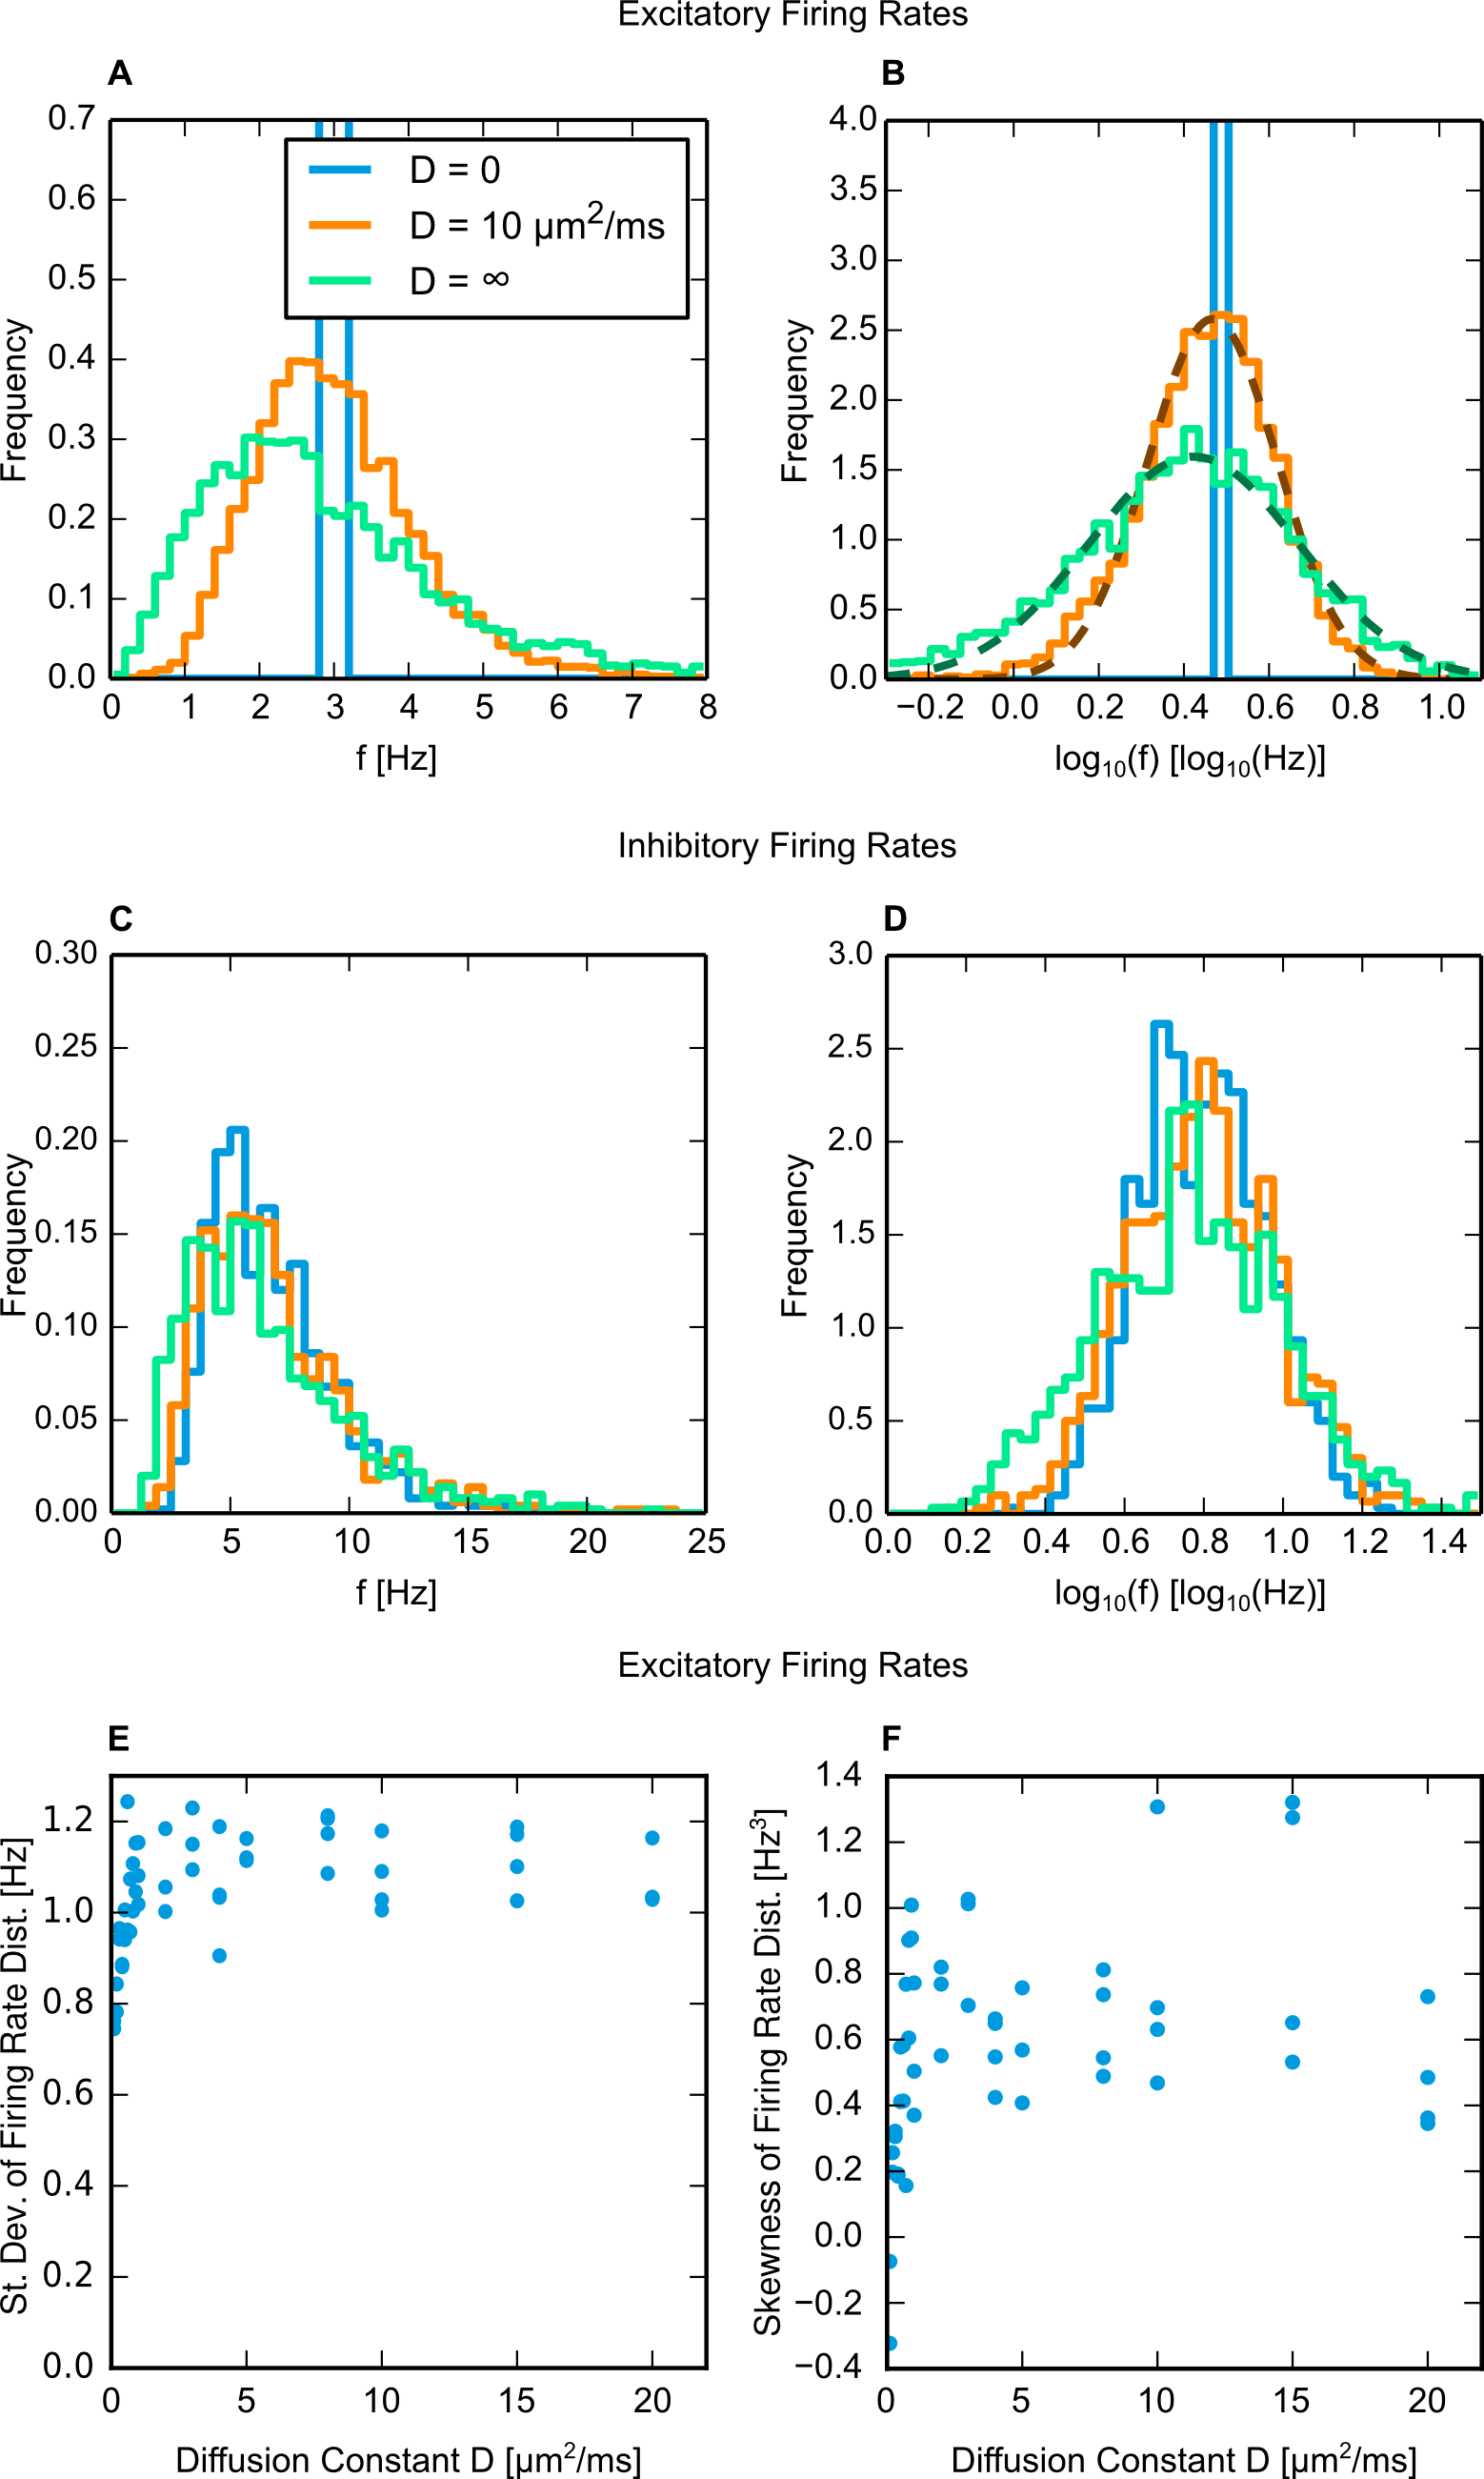
\includegraphics[width=0.9\textwidth]{./figures/fir_rate_dist_comp.png}
%\end{center}
\caption{{\bf Distribution of firing rates.} \textbf{A,B,C,D}: Empirical PDF of mean firing rates over the excitatory (A/B) and inhibitory (C/D) population in regular (A/C) and logarithmic space (B/D). Distributions were generated from 10 simulation runs, 1 simulation was used for non-diffusive homeostasis. Mean firing rates were calculated from spikes within $\mathrm{1000\,s} \leq t  \mathrm{\leq 1500\,s}$. Dashed lines in B are Gaussian fits. \textbf{E,F}: Standard deviation (E) and skewness (F) of firing rate distribution of excitatory neurons. Each data point was generated from one full simulation.}
\label{Fir_Rate_Dist_Comp}
\end{figure}

Sweeney et al. found that diffusive homeostasis maintains the variance of the distribution of firing rates across a wide range of diffusion constants but rapidly approaching zero for small values (cf. \cite{Sweeney_Paper}, Fig.~3C). We were able to reproduce this result, see Fig.~\ref{Fir_Rate_Dist_Comp}E. Homeostasis reaches a point of saturation, where faster diffusion has no effect on the heterogeneity of firing rates. Each of the data points in Fig.~\ref{Fir_Rate_Dist_Comp}E and F corresponds to a single full simulation, though the same simulation data was used in A and B. $\rm 55$ simulations were run in total. We picked the $\rm D$-values by hand to achieve a good representation of the overall trend while limiting the number of simulations. The set of diffusion constants used is given in Table \ref{Diff_Test_Constants_Sim_Number}.
%\begin{figure}
%\begin{center}
%\begin{minipage}{0.4\textwidth}
%%% freq_dist_width_vs_D.py
%\includegraphics[width=\textwidth]{../../plots/firing_rate_dists/std_dev_vs_D_neumann.png}
%\end{minipage}
%\begin{minipage}{0.4\textwidth}
%%% freq_dist_skew_vs_D.py
%\includegraphics[width=\textwidth]{../../plots/firing_rate_dists/skew_vs_D_neumann.png}
%\end{minipage}
%\end{center}
%\caption{{\bf Width and skewness of excitatory neurons' firing rates} Standard deviation (A) and skewness (B) of firing rate distribution of excitatory neurons (Neumann boundary conditions). Each data point was generated from one full simulation.}
%\label{Fir_Rate_Dist_Width_Skewness_vs_D}
%\end{figure}
We also investigated the influence of the diffusion constant on the distribution's skewness, shown in Fig.~\ref{Fir_Rate_Dist_Comp}F, to further quantify this dependence. Compared to the standard deviation, we saw a similar but not as clear trend with a drop for very small diffusion constants, even occasionally resulting in a left-skewed distribution (negative D-values).

\begin{table}[h]
\caption{\bf Diffusion constants and number of simulations used in Fig.~\ref{Fir_Rate_Dist_Comp}E and F.}
\begin{tabu}{|l|l|}
\hline
\boldmath{$\rm D\;[\upmu m^2 ms^{-1}]$} & \textbf{Number of Sim.} \\ \hline
$\rm 0.0$ & 1 \\ \hline
$\rm 0.1,0.2,...,0.8,0.9$ & 2 \\ \hline
$\rm 1.0,2.0,...,5.0,8.0,10.0,15.0,20.0$ & 4 \\ \hline
\end{tabu}
\label{Diff_Test_Constants_Sim_Number}
\end{table}

A naturally emerging question when altering the diffusion constant is how excitatory firing rates behave in the absolute limit of infinitely fast diffusion. In fact, this case is quite easy to implement in the simulation: One simply has to feed all NO sources into a single scalar variable of NO concentration. This then provided the same NO readout for all excitatory neurons, which means that all excitatory thresholds changed at the same rate all the time, only shifting their initial distribution. Therefore, the effect of this particalur distribution will remain present for the entire simulation, and a larger variance among excitatory thresholds will likely also broaden the distribution of firing rates. Even though the firing threshold is an abstract quantity and cannot be directly measured in biological neurons, analyses of neuronal voltage dynamics suggest that spike-initiation voltages in cortical neurons can vary on the order of tens of millivolts \cite{Azouz_2000, Jolivet_2006}. For simplicity however, we chose to set all excitatory thresholds to the same initial value. Fig.~\ref{Fir_Rate_Dist_Comp}A--D shows the distributions for this case. As one can see, this results in a similar but broader log-normal like distribution of excitatory firing rates, accompanied by a higher skewness of 1.51.

\subsection*{Model produces non-random features of network topology and dynamics}\label{Section_Topol_Preservation}
While we explicitly intended altering the statistics of excitatory firing rates by implementing diffusive homeostasis, we wanted to preserve what has previously been reported by Miner and Triesch regarding the evolution and structure of recurrent excitatory weights \cite{SORN_Paper}. More specifically, we were concerned with the following features of synaptic topology and dynamics: First, an overrepresentation of excitatory bidirectional connectivities, a feature found to be present in cortical networks \cite{Song_Connectivity_2005}. Second, a power-law distribution of synaptic lifetimes. Loewenstein et al. reported on this feature in a study on the auditory cortex of mice \cite{Loewenstein_2015}. Third, a heavy-tailed, log-normal like distribution of synaptic efficacies, which have been observed in a number of experimental studies\cite{Song_Connectivity_2005,Yasumatsu_Synapses_2008,Lefort_2009,Loewenstein_Spine_Sizes}.

Figure~\ref{Syn_Topology_Features} summarizes the results regarding these properties. As shown in Fig.~\ref{Syn_Topology_Features}A and B, Diffusive homeostasis leads to the same stable level of recurrent excitatory connection fraction, as well as an over-representation of bidirectional connections. This over-representation is due to the distance-dependent probability of creating a new synapse between a pair of excitatory neurons \cite{SORN_Paper,Hoffmann_2017}.

Figure~\ref{Syn_Topology_Features}C shows that a log-normal like distribution of excitatory weights is preserved under diffusive homeostasis. 
Theoretical approaches to explaining this property are mainly based on a combination of multiplicative and additive weight dynamics \cite{Loewenstein_Spine_Sizes,Pengsheng_2013,Statman_Synapses_2014,Loewenstein_2015}, which
is in line with our implementation of multiplicative normalization and additive STDP.

Figure~\ref{Syn_Topology_Features}D illustrates the preservation of a power-law distribution of recurrent excitatory synaptic lifetimes during the steady phase of connectivity. The precise slope of the power law has previously been related to the balance of potentiation and depression \cite{SORN_Paper}.

\begin{figure}[h]
%\begin{center}
%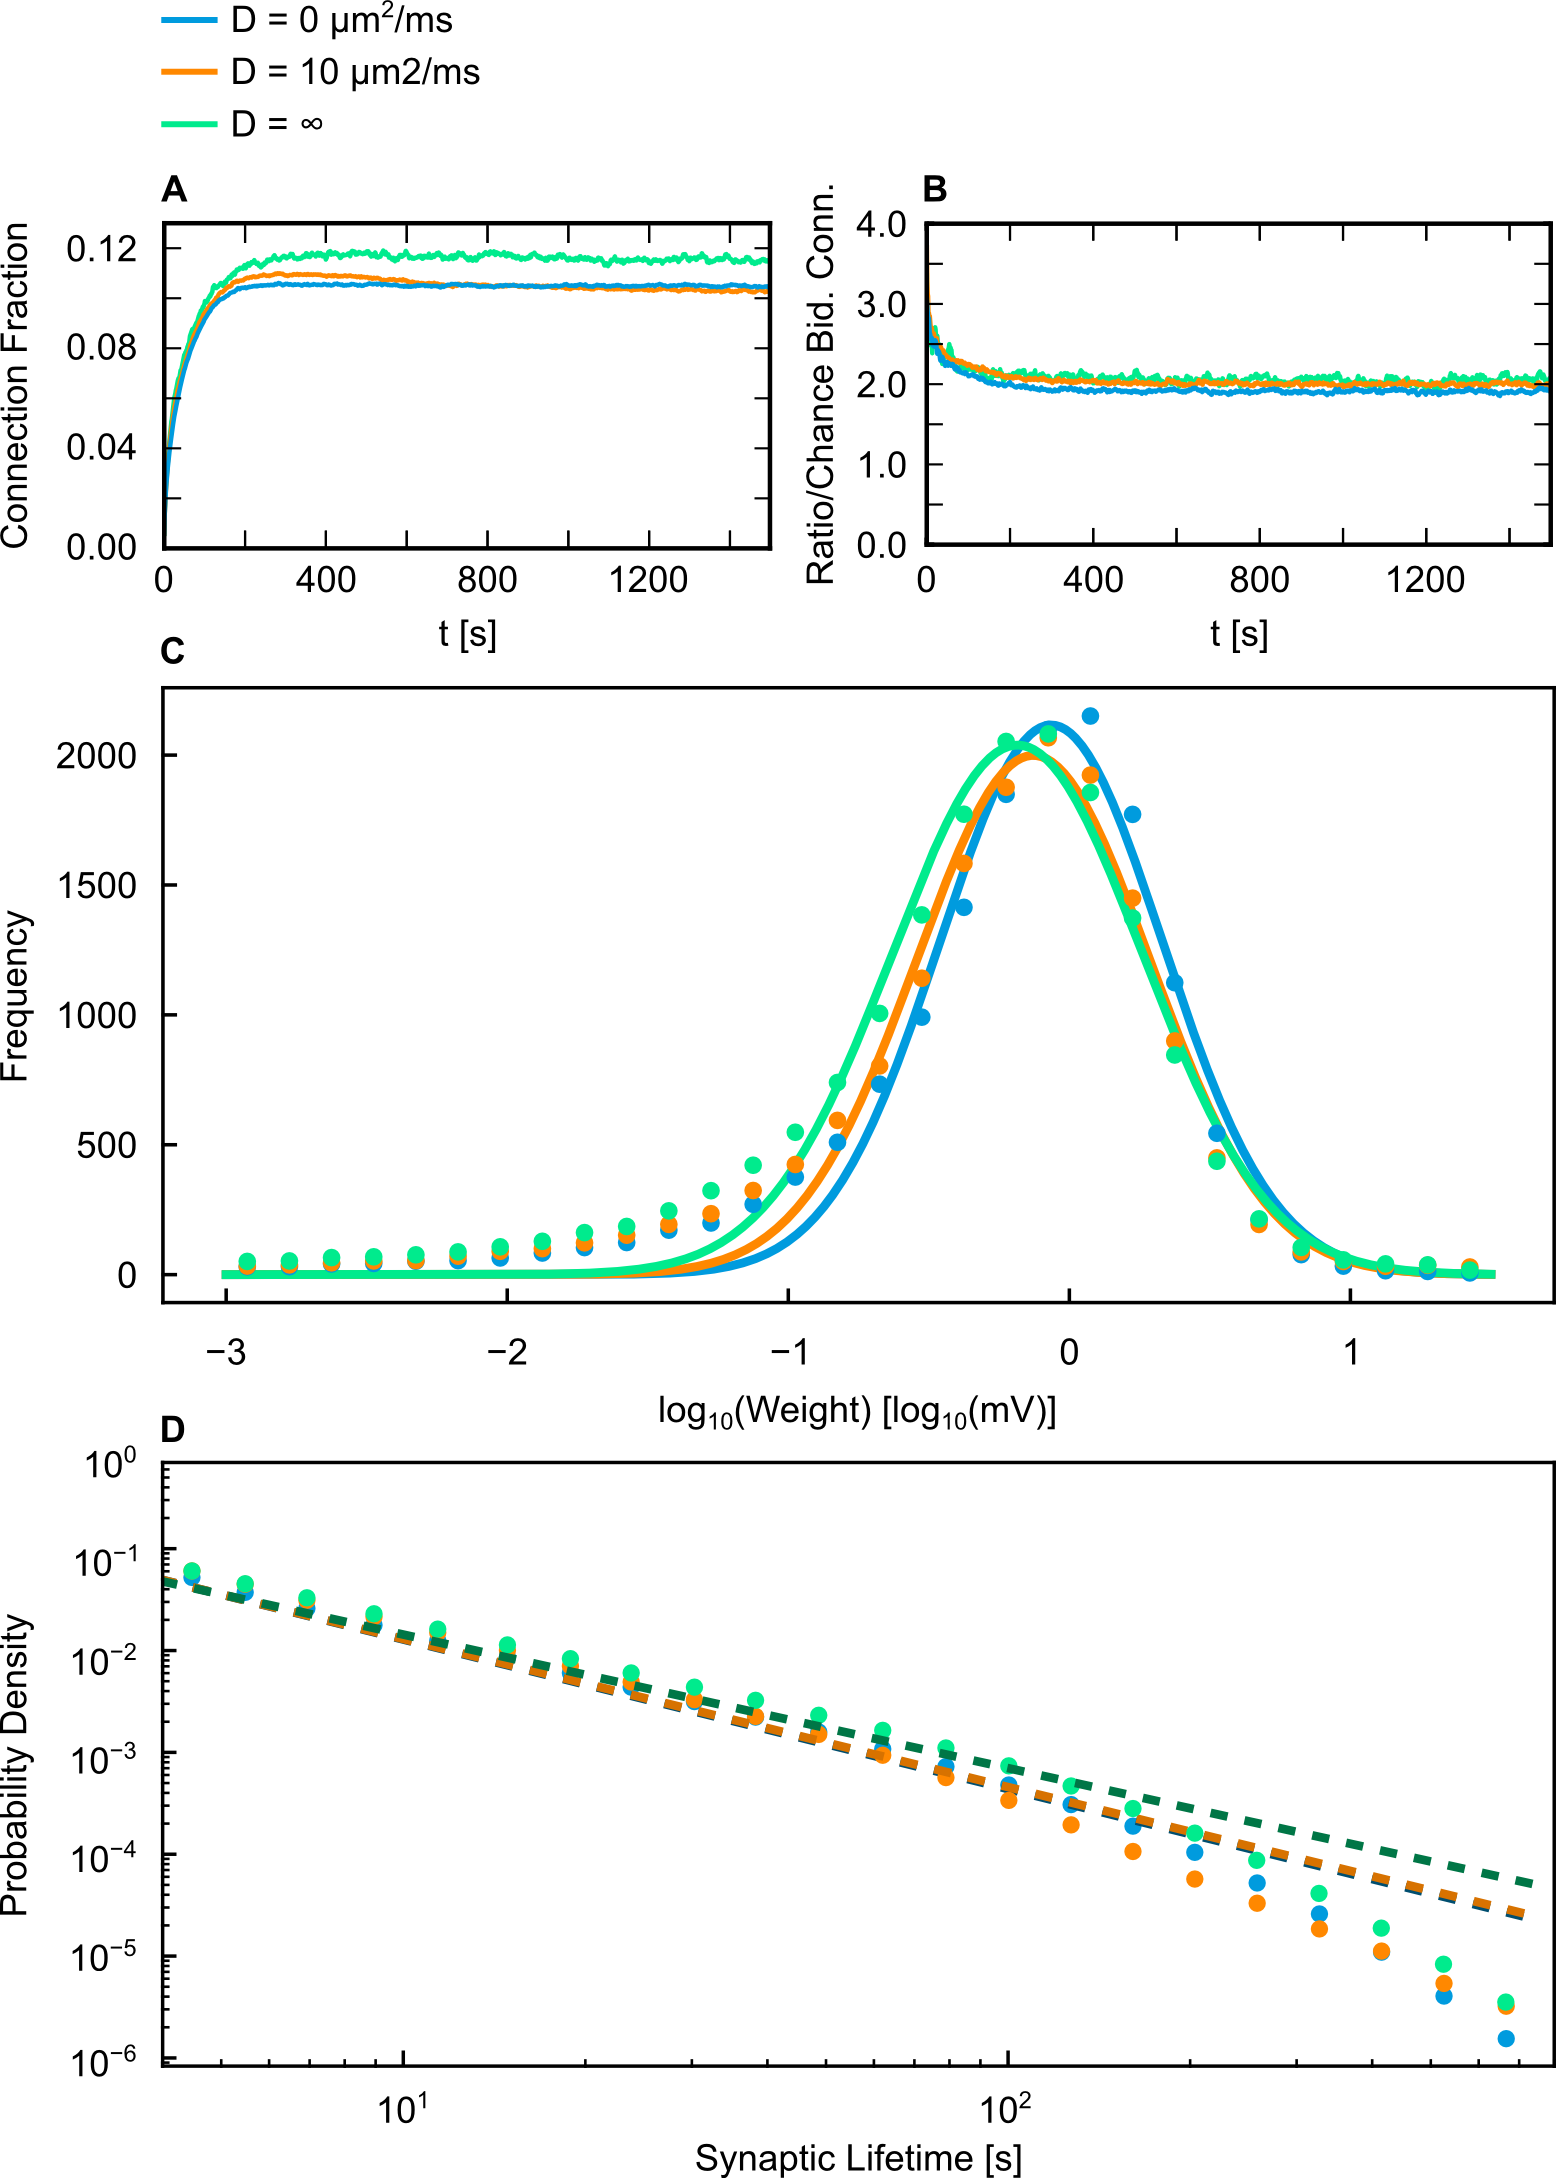
\includegraphics[width=\textwidth]{./figures/syn_topology_comp.png}
%\end{center}
\caption{{\bf Structural and dynamic features of excitatory synaptic connectivity.} \textbf{A}: Evolution of recurrent excitatory connection fraction. \textbf{B}: Ratio of bidirectional connections relative to a random Erd\H{o}s-Renyi graph. \textbf{C}: Distribution of excitatory recurrent weights after $\rm 1500\, s$. Solid curves are Gaussian fits. Data for each diffusion constant was taken from 5 simulations. \textbf{D}: Distribution of recurrent excitatory synaptic lifetimes. Single-trial data. Solid lines are estimates of a power-law exponent, giving a slope of approximately $\mathrm{-1.9}$ for diffusive homeostasis and $\mathrm{-1.7}$ for non-diffusive homeostasis. 5 simulation runs were used for each curve in panels A and B, panels C and D show representative single-trial data.}
\label{Syn_Topology_Features}
\end{figure}
\subsection*{Heterogeneity of firing rate leads to the emergence of strongly influential excitatory neurons}\label{Section_Mean_outgoing_Weights}
Having established that the model accounts for above-chance bidirectional connectivities, a log-normal like distribution of recurrent excitatory weights and a power-law distribution of synaptic lifetimes in the same way as its predecessor, we sought for possible differences within our network topology as a result of diffusive homeostasis. Since we only implemented synaptic normalization for the sum of incoming weights, the total or average strength of \emph{outgoing} connections may vary from cell to cell. In a sense, the strength of outgoing connections per neuron can be regarded as a measure of how influential a neuron's activity is with respect to other neurons in the network. Effenberger et al. have proposed a model where such ``driver neurons" form highly active and interconnected subnetworks \cite{Effenberger_2015}, an observation that is backed up by experimental studies \cite{Yassin_Subnetworks_2010,Eckmann_Leader_Neurons_2008}. Figure \ref{Outgoing_Weights_Comp}A shows that diffusive homeostasis allows for the emergence of a small group of highly influential neurons, which resembles the findings in \cite{Effenberger_2015}. A comparison of statistics generated with shuffled versions of the weight matrices shows that above-chance exceptionally strong mean outgoing weights were indeed present (two-sample Kolmogorov-Smirnov test, $p < 10^{-30}$).

\begin{figure}[h]
%%% plot_sum_outgoing_weights_dist.py
%%% out_weight_vs_f.py
%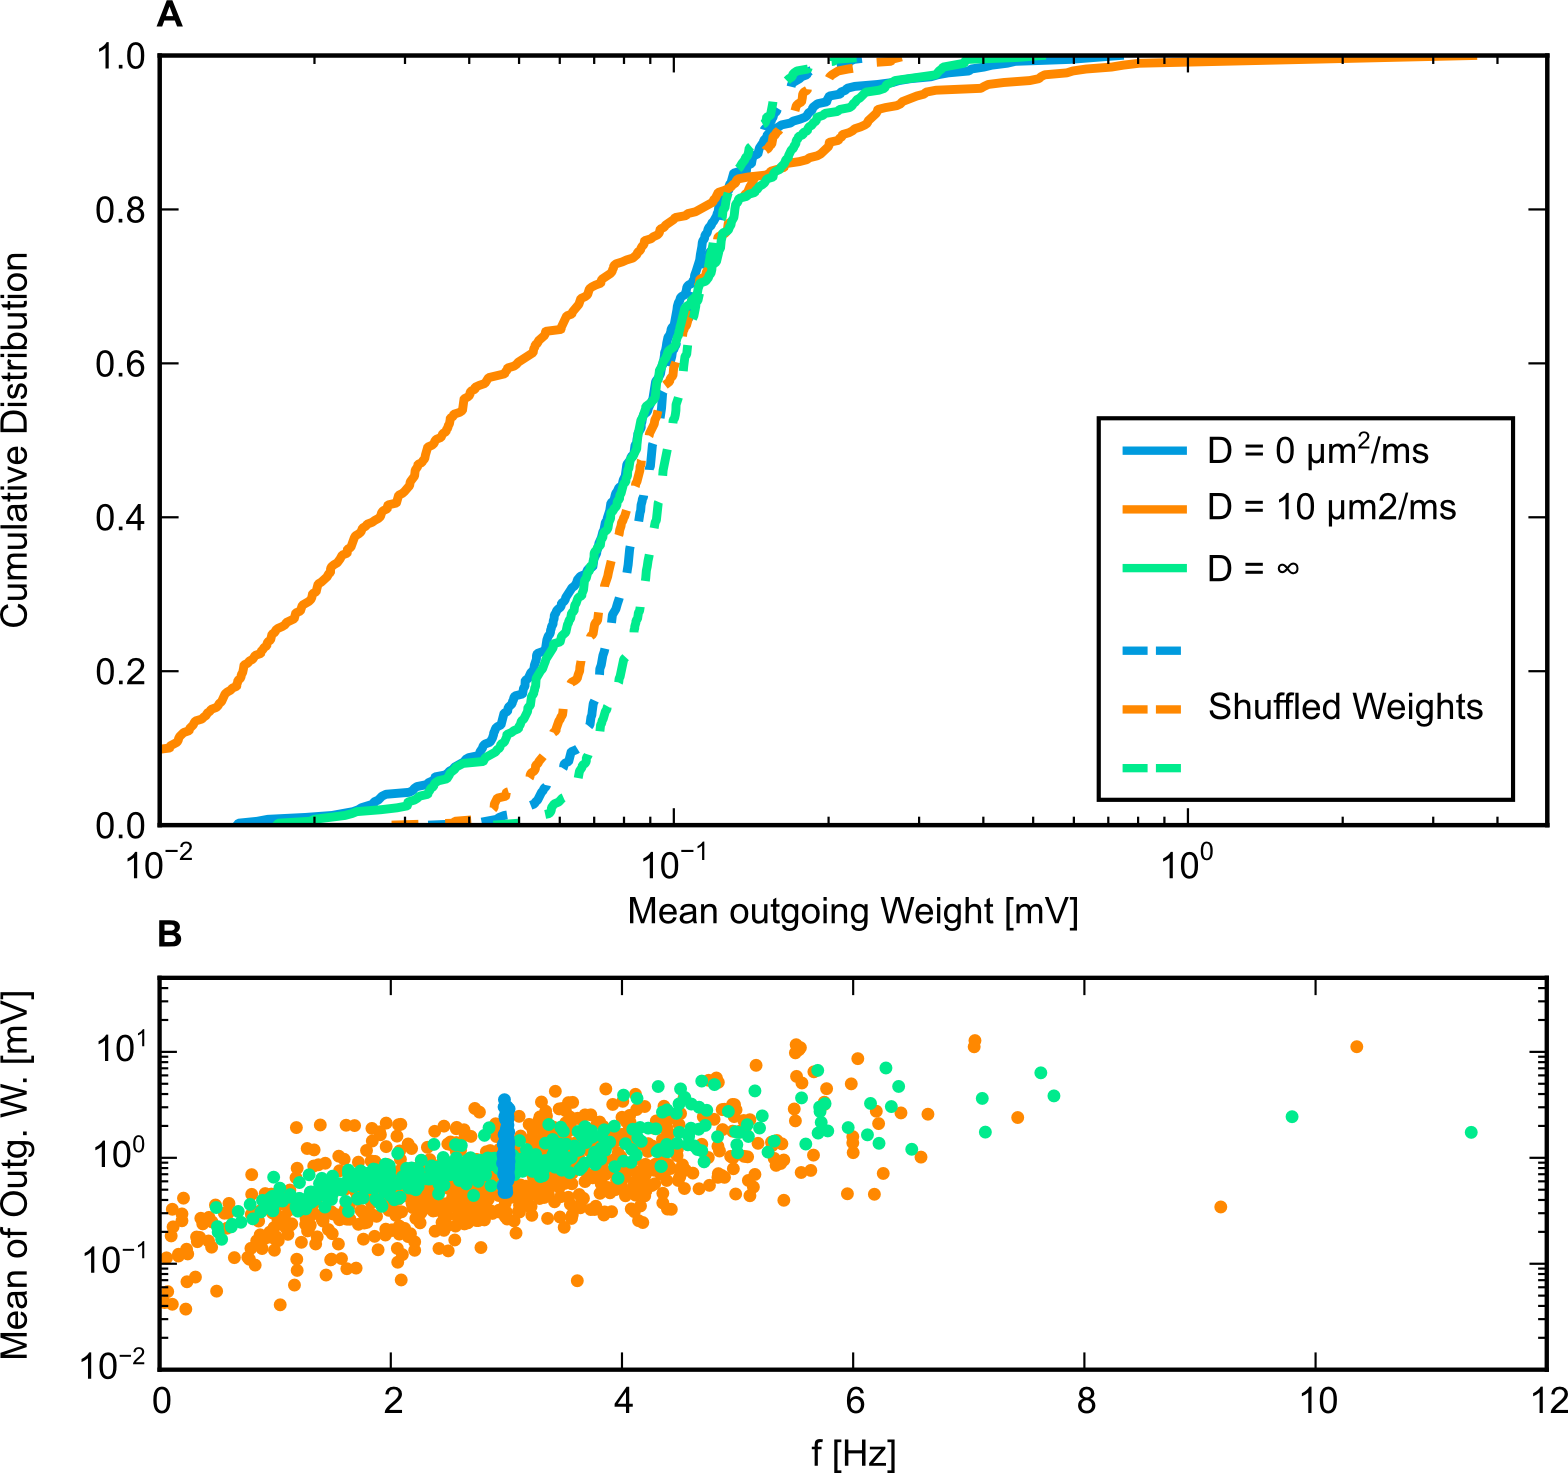
\includegraphics[width=\textwidth]{./figures/outgoing_weights_comp_new_cumsum.png}
\caption{{\bf Presence of strongly influential neurons with high firing rates.} \textbf{A}: Cumulative distribution of decadic logarithm of mean outgoing excitatory weights. Dashed lines are means obtained by randomly shuffling synaptic weights. Single trial data. \textbf{B}: Mean of outgoing excitatory weights at $t=\mathrm{1500\,s}$ plotted against mean presynaptic firing rate (averaged over $\mathrm{700\,s \leq} t \mathrm{ \leq 1000\,s}$) in logarithmic space. Each point corresponds to a presynaptic excitatory cell. Two simulation runs were used for diffusive homeostasis, all other are single-trial data.}
\label{Outgoing_Weights_Comp}
\end{figure}

Synapses between highly active presynaptic cells and postsynaptic neurons with lower activity are known to be subject to long-term potentiation \cite{Sjoestroem_Syn_Plasticity_2001,Feldman_STDP_2012}. With this causal relation in mind, we argue that diffusive homeostasis effectively embodies a similar functional role as inhibitory STDP in \cite{Effenberger_2015} by allowing for the presence of excitatory cells with strongly above-average activity. We tested this relationship by plotting the mean outgoing weights against the average firing rate, see Fig.~\ref{Outgoing_Weights_Comp}B. A strong heterogeneity of firing rates allowed for the development of few neurons with comparably strong mean outgoing weights, while the distribution of mean weights resulting from a narrow distribution is limited to a smaller range. We also tested the case of instantaneous diffusion. Mean weights did not reach as high values as in the case of diffusion at a finite rate.

Experimental studies have not only considered the presence of neurons with strong influence onto other neurons \cite{Eckmann_Leader_Neurons_2008}, but also found evidence that highly active neurons form subnetworks with an increased connectivity, in the sense that these cells are more likely than average to connect to each other, see \cite{Yassin_Subnetworks_2010}. We tested this in our network by evaluating the connection fraction among the top 10\% of excitatory neurons with respect to their average firing rate within $\mathrm{1000\,s} \leq t \leq \mathrm{1500\,s}$ and comparing it to the rest of the excitatory population and the same calculation for the non-diffusive case. This returned $\rm CF= 0.1371 \pm 0.0061$ for the top 10\% and $\rm CF = 0.0982 \pm 0.0013$ for the lower 90\% in the case of diffusive homeostasis, and  $\rm CF = 0.0954 \pm 0.0044$ for the top 10\% and $\rm CF = 0.0992 \pm 0.0002$ for the lower 90\% in the case of non-diffusive homeostasis. Standard errors were calculated from 5 simulation runs for each homeostatic mechanism, and connectivity matrices were taken from $t = \mathrm{1500\,s}$. This difference was significant only in the case of diffusive homeostasis (Welch's t-test, $\rm p = 3.87 \times 10 ^ {-3}$ for diffusive homeostasis, $\rm p = 0.48$ for non-diffusive homeostasis). Effenberger et al. reported a similar effect, in fact with even more pronounced differences of connectivity \cite{Effenberger_2015}.

\subsection*{Spatial configuration of neurons allows for the precise prediction of firing rates}\label{Section_Rand_Mat_vs_Sim}
Having analyzed the distribution of firing rates resulting from the implementation of diffusive homeostasis, we were interested in how strongly the actual positioning of excitatory neurons influences the resulting statistics of firing activity. To do so, we assumed that the spontaneous firing measured during the stable phase of the network, characterized by a constant excitatory connection fraction, can be regarded as a homeostatic steady state. Given no sudden strong changes of neural input, the homeostatic feedback levels out the error signal, given by ${\rm [NO]} - {\rm [NO]}_0$ to approximately zero, since \eqref{Theta_dyn} is a realization of an integral control. Our search for the steady-state configuration of firing rates thus reduced to finding a set of firing rates that led to a concentration level of ${\rm [NO]}_0$ at every excitatory neuron's position:
\begin{equation}
{\rm [NO]}(\mathbf{x}_{i}) = {\rm [NO]}_0 \:, \: \forall i \; .
\label{NO_equil_cond}
\end{equation}
Furthermore, we found that the nonlinearity between spiking activity and NO synthesis could be well approximated by a linear relation between average firing rate $r_i$ and rate of NO synthesis $nNOS_i$ by
\begin{equation}
{\rm [nNOS]}_i = \frac{{\rm [Ca^{2+}]}^3_{\rm spike} \tau_{\rm Ca^{2+}}\ln(2)}{3} r_i \equiv \gamma r_i \; .
\label{simpl_nNOS}
\end{equation}
See Appendix S1 for a derivation of the proportionality factor. Given this simplification, the steady state of NO concentration is thus defined by the solution of
\begin{equation}
0 =-\lambda {\rm [NO]} + D \nabla^2 {\rm [NO]} + \sum_{i} \delta^2(\mathbf{x}-\mathbf{x}_{i}) \gamma r_i \label{simple_NO_dyn_with_diff}
\end{equation}
which can be reformulated to
\begin{equation}
\left(\nabla^2 + \left( i\sqrt{\frac{\lambda}{D}}\right)^2\right) {\rm [NO]} = \sum_{i} \delta^2(\mathbf{x}-\mathbf{x}_{i}) \frac{- \gamma r_i}{D}
\label{simple_NO_dyn_with_diff_equil_helmholtz}
\end{equation}
which is a two-dimensional Helmholtz equation. Its Green's function is
\begin{equation}
{\rm [NO]}(\mathbf{x}) = \frac{r_i \gamma}{2 \pi D} K_0 \left(|\mathbf{x}|\sqrt{\frac{\lambda}{D}} \right) \equiv r_i  \psi_{\rm point}(|\mathbf{x}|)
\label{solution_diff_equil_bessel}
\end{equation}
where $\mathrm{K_0}$ is the zeroth modified Bessel function of the second kind \cite{Helmholtz_Solution_2d}.  This solution reveals a fundamental problem of modeling the sources of NO production as point sources: the fact that $\mathrm{K_0(x)}$ diverges to infinity for $\mathrm{x\rightarrow 0}$. It is merely due to the finite density of the numeric grid used for the simulation of diffusion that allows for a finite target value of concentration.

Generally speaking, no matter how the actual shape of the numeric solution in the equilibrium at a constant production rate looks like, it must be of the form
\begin{equation}
{\rm [NO]}_i(\mathbf{x}) = r_i  \psi (|\mathbf{x}_{i}-\mathbf{x}|) \;  . \label{general_diff_interaction}
\end{equation}
The full solution is then
\begin{equation}
{\rm [NO]}(\mathbf{x}) = \sum_i {\rm [NO]}_i(\mathbf{x})\;.
\label{full_sol_diff_equil}
\end{equation}
By defining
\begin{equation}
\psi_{ij} \equiv \psi_{ji} \equiv \psi (|\mathbf{x}_i-\mathbf{x}_j|)
\label{interact_matrix_elements}
\end{equation}
we could express condition \eqref{NO_equil_cond} as
\begin{equation}
\sum_j \psi_{ij} r_j = {\rm [NO]}_0
\label{NO_equil_cond_interact_matrix}
\end{equation}
or, as an operator
\begin{align}
\hat{\psi}\mathbf{r} &= {\rm [NO]}_0 \mathbf{n} \label{NO_equil_cond_interact_matrix_operator} \\
\mathbf{n}&\equiv (1,1,...,1) \; .
\end{align}
The problem of finding the steady-state solution of the homeostatic constraint thus reduced to inverting $\hat{\psi}$:
\begin{equation}
\mathbf{r} = {\rm [NO]}_0 \hat{\psi}^{-1} \mathbf{n} \; .
\label{NO_euqil_cond_interact_matrix_operator_solve}
\end{equation}

Still, we had to find a modified, non-diverging version of $\mathrm{\psi (d(\mathbf{x}_{\mathrm{neur.},i},\mathbf{x}))}$ to acquire any prediction from this model. It had to retain the shape given by \eqref{solution_diff_equil_bessel} for larger distances but approach the correct numeric error value at the origin, determined by the spacing of the numeric grid. We solved this problem by the following expression:
\begin{equation}
\psi_{\rm approx.} \equiv \frac{1}{\left(\frac{1}{\psi_0^\varepsilon} + \frac{1}{\psi_{\rm point}^\varepsilon}\right)^{\frac{1}{\varepsilon}}}
\label{Numeric_Solution_Expression_Trick}
\end{equation}
where $\mathrm{\varepsilon}$ determines the ``smoothness" of transition between $\mathrm{\psi}$ and the cutoff value $\mathrm{\psi_0}$. We chose $\mathrm{\varepsilon=10}$ for all further calculations. We took the simple approach of interpreting this value as a mean of the analytic solution across the area covered by the corresponding grid cell to find an expression for $\mathrm{\psi_0}$. As an additional simplification, we substituted the necessary integration over the square grid cell by a circular area of equal size around the source. This calculation yielded
\begin{equation}
\psi_0 = \gamma \frac{1-h\sqrt{\frac{\lambda}{\pi D}} K_1\left( h\sqrt{\frac{\lambda}{\pi D}}\right) }{h^2 \lambda}
\label{Numeric_Grid_Bessel_Approx}
\end{equation}
where $\mathrm{h}$ is the spatial resolution of the grid cells.

By simply calculating all matrix elements of $\mathrm{\hat{\psi}}$ by means of \eqref{interact_matrix_elements}, one would neglect the finite boundaries of the system, which would cause neurons close to the edge to ``bleed" into empty space. We accommodated for zero-flux Neumann boundary conditions by adding appropriately mirrored copies of the neurons' positions, canceling the orthogonal component of the gradient at the boundaries. 

After having worked out the analytical basis, we compared the prediction obtained from numerically solving \eqref{NO_equil_cond_interact_matrix_operator} for certain spatial configurations of neurons to the steady-state firing rates of the full spiking network with the same spatial structure. As Fig.~\ref{Matrix_Predict_Comp}A shows, the actual shape of the distribution was well predicted by the solution of the linear system. Furthermore, we were particularly interested in the quality of the predictions with respect to the choice of diffusion constant. Fig.~\ref{Matrix_Predict_Comp}B shows three examples: For $\mathrm{D=10\, \upmu m^2 ms^{-1}}$, the correlation between measured and predicted firing rates is very good. In contrast, we included the --- obviously unsuccessful --- attempt to predict firing rates for a simulation with instantaneous diffusion based on the spatial structure by setting D to a relatively high value of $\mathrm{D=100\, \upmu m^2 ms^{-1}}$. This represented a limiting case where our analytic model could not make any meaningful predictions, since instantaneous diffusion overrides any spatial inhomogeneities. The outcome of the third case shown in the plot, $\mathrm{D=0}$, is correctly predicted by the analytic model. In general, instantaneous diffusion as well as $\mathrm{D=0}$ overrode the effects of spatial heterogeneity onto firing rates. 

\begin{figure}[h]
%% fir_dist_shape_sim_matrix_compare.py
%% plot_rand_matrix_sol_vs_sim.py
%% sim_vs_matrix_solve_corr_vs_D.py
%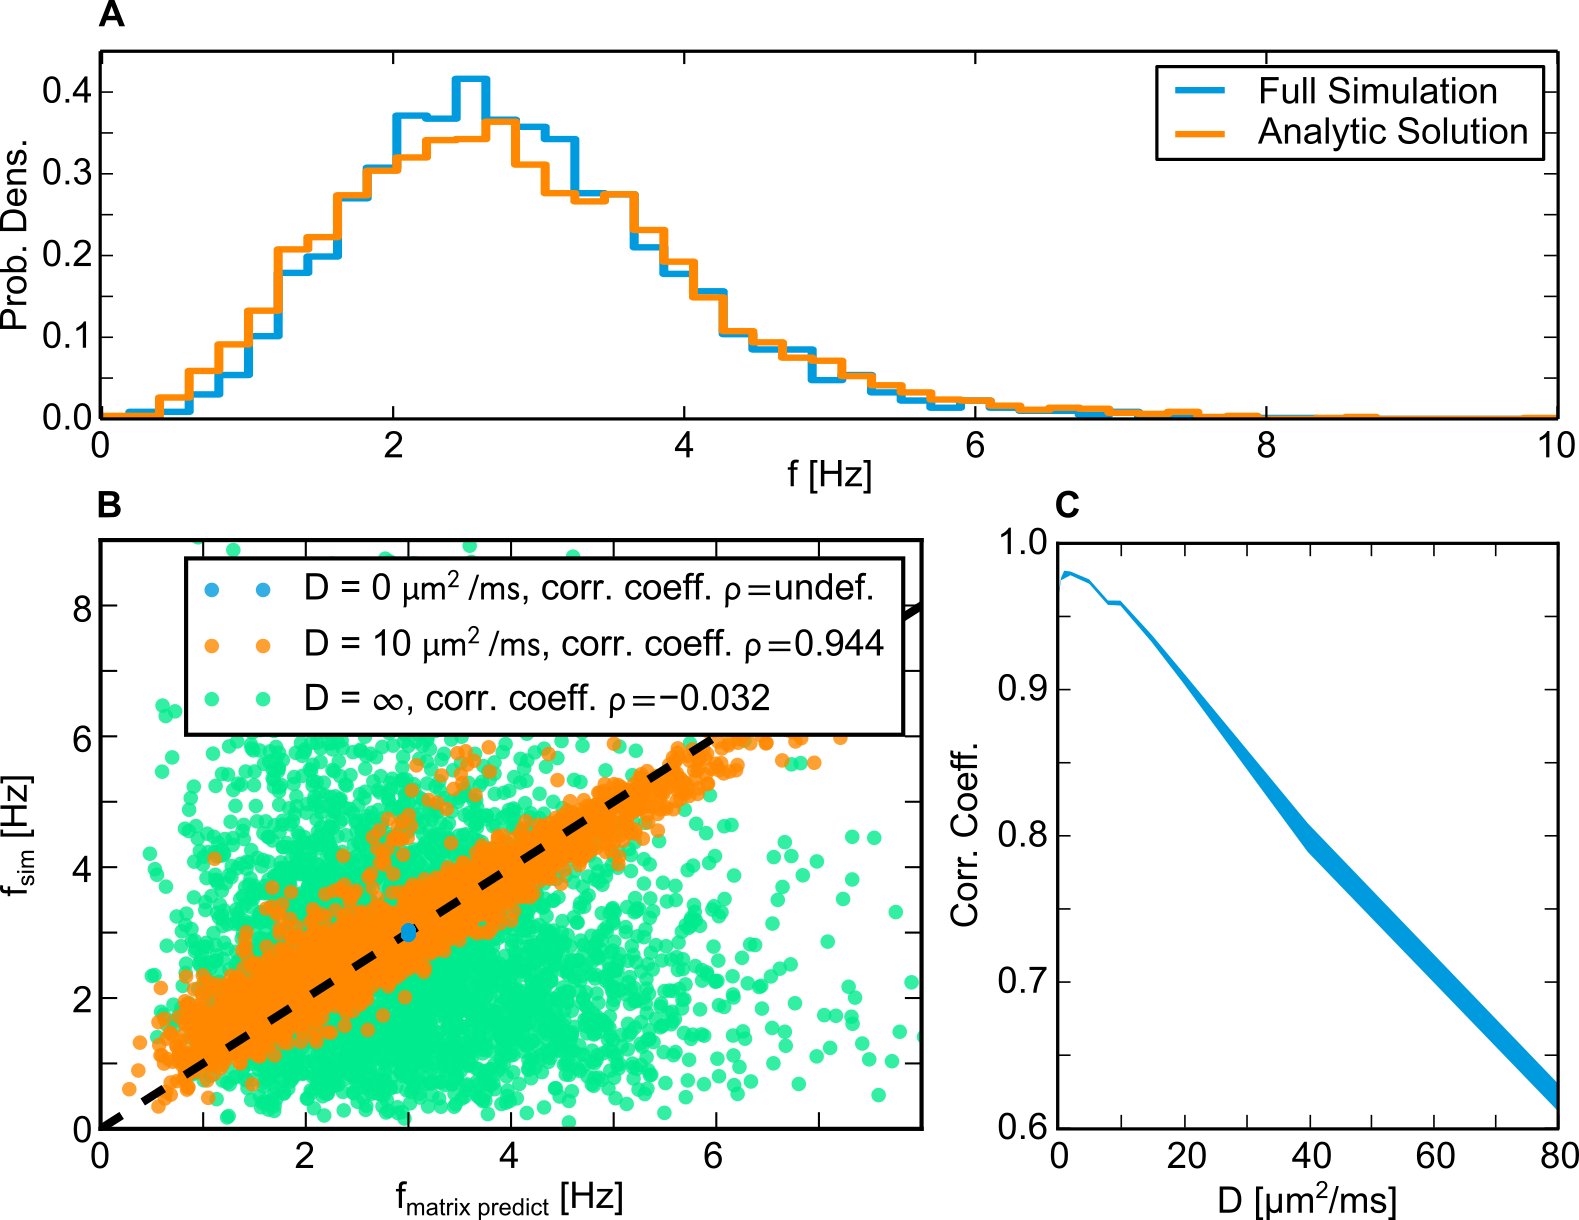
\includegraphics[width=\textwidth]{./figures/matrix_predict_comp_figure_new.png}
\caption{{\bf Empirical distribution of excitatory firing rates and theoretical prediction.} \textbf{A}: Distribution of firing rates for $\mathrm{D=10\, \upmu m^2 ms^{-1}}$, full simulation and analytic prediction. Data was taken from 10 simulation runs. \textbf{B}: Measured firing rates ($\mathrm{ 1000\,s} \leq t \leq \mathrm{1500\, s}$) versus predicted firing rates based on the solution of  \eqref{NO_equil_cond_interact_matrix_operator}. For $\mathrm{D=\infty}$ (instantaneous diffusion in the full simulation), the analytic prediction was calculated with a comparably large diffusion constant of $\mathrm{D=100\, \upmu m^2 ms^{-1}}$. Plot shows representative single-trial data. \textbf{C}: Pearson correlation coefficient of predicted and measured firing rates versus diffusion constant. Line width depicts standard error, 5 simulations were used for each $\rm D$-value.}
\label{Matrix_Predict_Comp}
\end{figure}

These observations naturally led us to the question of how the correlation between predicted and measured firing rates behaves in between the aforementioned limits. Especially, we were interested in the range of the diffusion constant for which our model provides a good description of the full spiking network's activity. Fig.~\ref{Matrix_Predict_Comp}C depicts the Pearson correlation coefficient of $\mathrm{f_{\rm matrix, predict.}}$ and $\mathrm{f_{\rm sim.}}$ against the diffusion constant used in the simulation. A relatively high correlation was obtained for a wide range of diffusion constants. However, we could see a general decline of correlation for larger diffusion constants. This trend was in line with the aforementioned limit of instantaneous diffusion, namely a complete decorrelation between prediction and measurement, as well as the good agreement for $\mathrm{D= 10\, \upmu m^2 ms^{-1}}$ shown in Fig.~\ref{Matrix_Predict_Comp}A.

Having acknowledged the good agreement between the full network simulation and the predictions of our simplified model, we also made predictions for more realistic settings of spatial densities. Although neuronal densities can vary considerably across different cortical areas and species \cite{Collins_2010}, we considered a density of $\rm 9\times 10^4\, mm^{-3}$ as a realistic value \cite{Schuez_1989}. This corresponds to a mean free path of $\rm 22.31 \upmu m$. On a single two-dimensional slice of $\rm 1000\, \upmu m \times 1000\, \upmu m$, one should therefore populate approximately $2000$ neurons to achieve the same mean free path. For the sake of a larger sample set, we calculated the homeostatic equilibrium for $8000$ randomly placed cells on a $\rm 2000\, \upmu m \times 2000\, \upmu m$ sheet. As shown in Fig.~\ref{Large_Diff_Test} (blue histogram), this resulted in an equally shaped, skewed distribution of firing rates.  

\begin{figure}[h]
%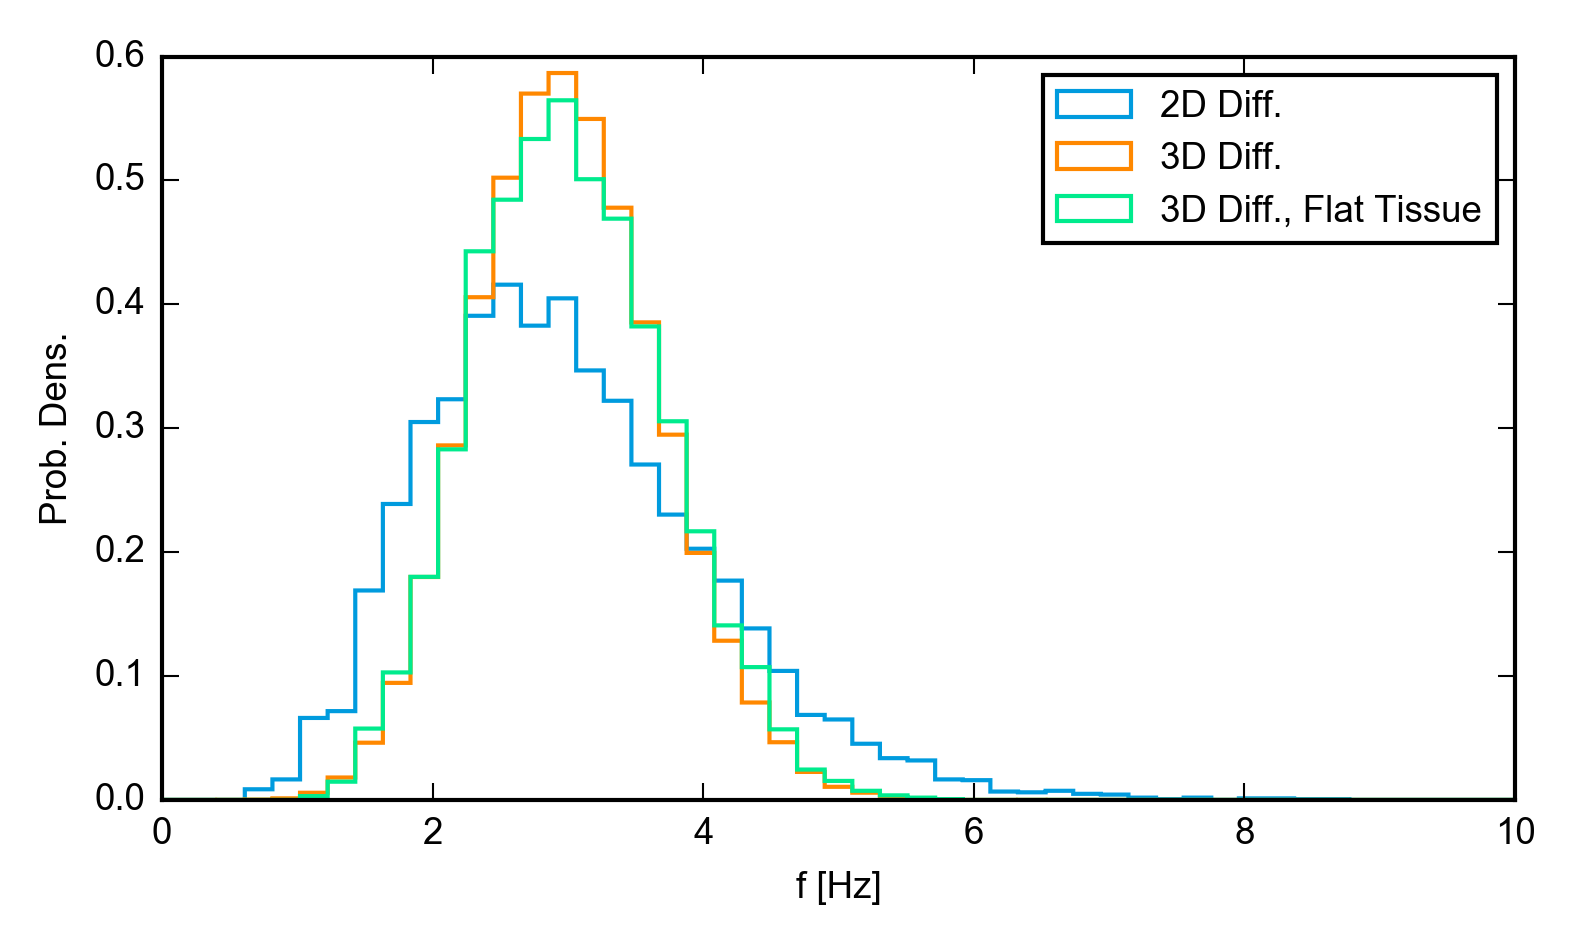
\includegraphics[width=\textwidth]{./figures/diff_test_combined.png}
\caption{Distribution of firing rates acquired by solving the diffusive homeostatic fixed point. 2D variant was carried out on a $\rm 2000\, \upmu m \times 2000\, \upmu m$ sheet (grid resolution $\rm 200 \times 200$) and $8000$ randomly picked cell positions. 3D variant used a $\rm 1000\, \upmu m \times 1000\, \upmu m \times 1000\, \upmu m$ cube (grid resolution $\rm 100 \times 100 \times 100$) and $\rm 9\times 10^4$ random cell positions. The 3D variant with a flat neural tissue used a $\rm 2000\, \upmu m \times 2000\, \upmu m \times 1000\, \upmu m$ cube (grid resolution $\rm 200 \times 200 \times 100$) and $8000$ cell positions with random x- and y-coordinates and a z-coordinate fixed at $\rm 500\, \upmu m$. All graphs depict single-trial data.}
\label{Large_Diff_Test}
\end{figure}

Two other variants of diffusion and cell placement are also shown in Fig.~\ref{Large_Diff_Test}: $9\times 10^4$ randomly placed cells in a cube of $\rm 1\, mm^3$, and a single, flat layer of $8000$ cells (random x- and y-position, fixed z-coordinate) in a $\rm 2000 \, \upmu m \times 2000 \, \upmu m \times 1000 \, \upmu m$ cuboid. While the former case mimics a uniform neuronal structure, the latter was meant to mimic interaction solely across a single cortical layer. All other diffusion parameters ($\lambda$ and $D$) were kept at their standard values. The resulting firing rate distributions are depicted in Fig.~\ref{Large_Diff_Test}. Both variants in 3D space yielded similar distributions, which, however, differed from the original setup with respect to variance and skewness, both being reduced.

Given the good predictions of firing rates of our simplified mathematical model under the standard configuration, these additional predictions suggest the implementation of a full network simulation combined with 3D diffusion for further testing of the homeostatic model. Apparently, the fact that diffusion in three dimensions results in a more localized fundamental solution of a single point source compared to two dimensions leads to a reduced intercellular overlay of homeostatic signals. We also noticed that the width of the distributions could not be further broadened artificially by increasing the the diffusion constant to very high values.


\subsection*{Low-density neighborhoods correlate with strong outgoing connections}
We previously stated that diffusive homeostasis allowed the network to develop few neurons with exceptionally strong outgoing weights. We found this effect to be present in neurons with a highly above-average firing rate. Moreover, our analytical predictions of individual neuronal activity suggest that the steady state of firing rates is strongly influenced by the spatial structure of excitatory neurons. Combining these two qualities led us to the conclusion that one should be able to observe some relation between spatial structure and the emergence of ``driver neurons". More specifically, regions of neurons with above average firing rates should develop stronger outgoing connections. We approximated the local neuron density by means of a Gaussian kernel with $\mathrm{\sigma = 50\, \upmu m}$ to test this hypothesis. Fig.~\ref{Inverse_Dens_vs_Sum_Out_Weights} shows the results. Despite a certain amount of randomness, our prediction was indeed verified. 
\begin{figure}[h]
%% density_vs_sum_out_weights.py
%\begin{center}
%\includegraphics[width=0.5\textwidth]{../../plots/scatter_density_out_weights_new.png}
%% density_vs_sum_out_weights_points.py
%\includegraphics[width=0.5\textwidth]{../../plots/scatter_density_out_weights_points_new.png}
%\end{center}
%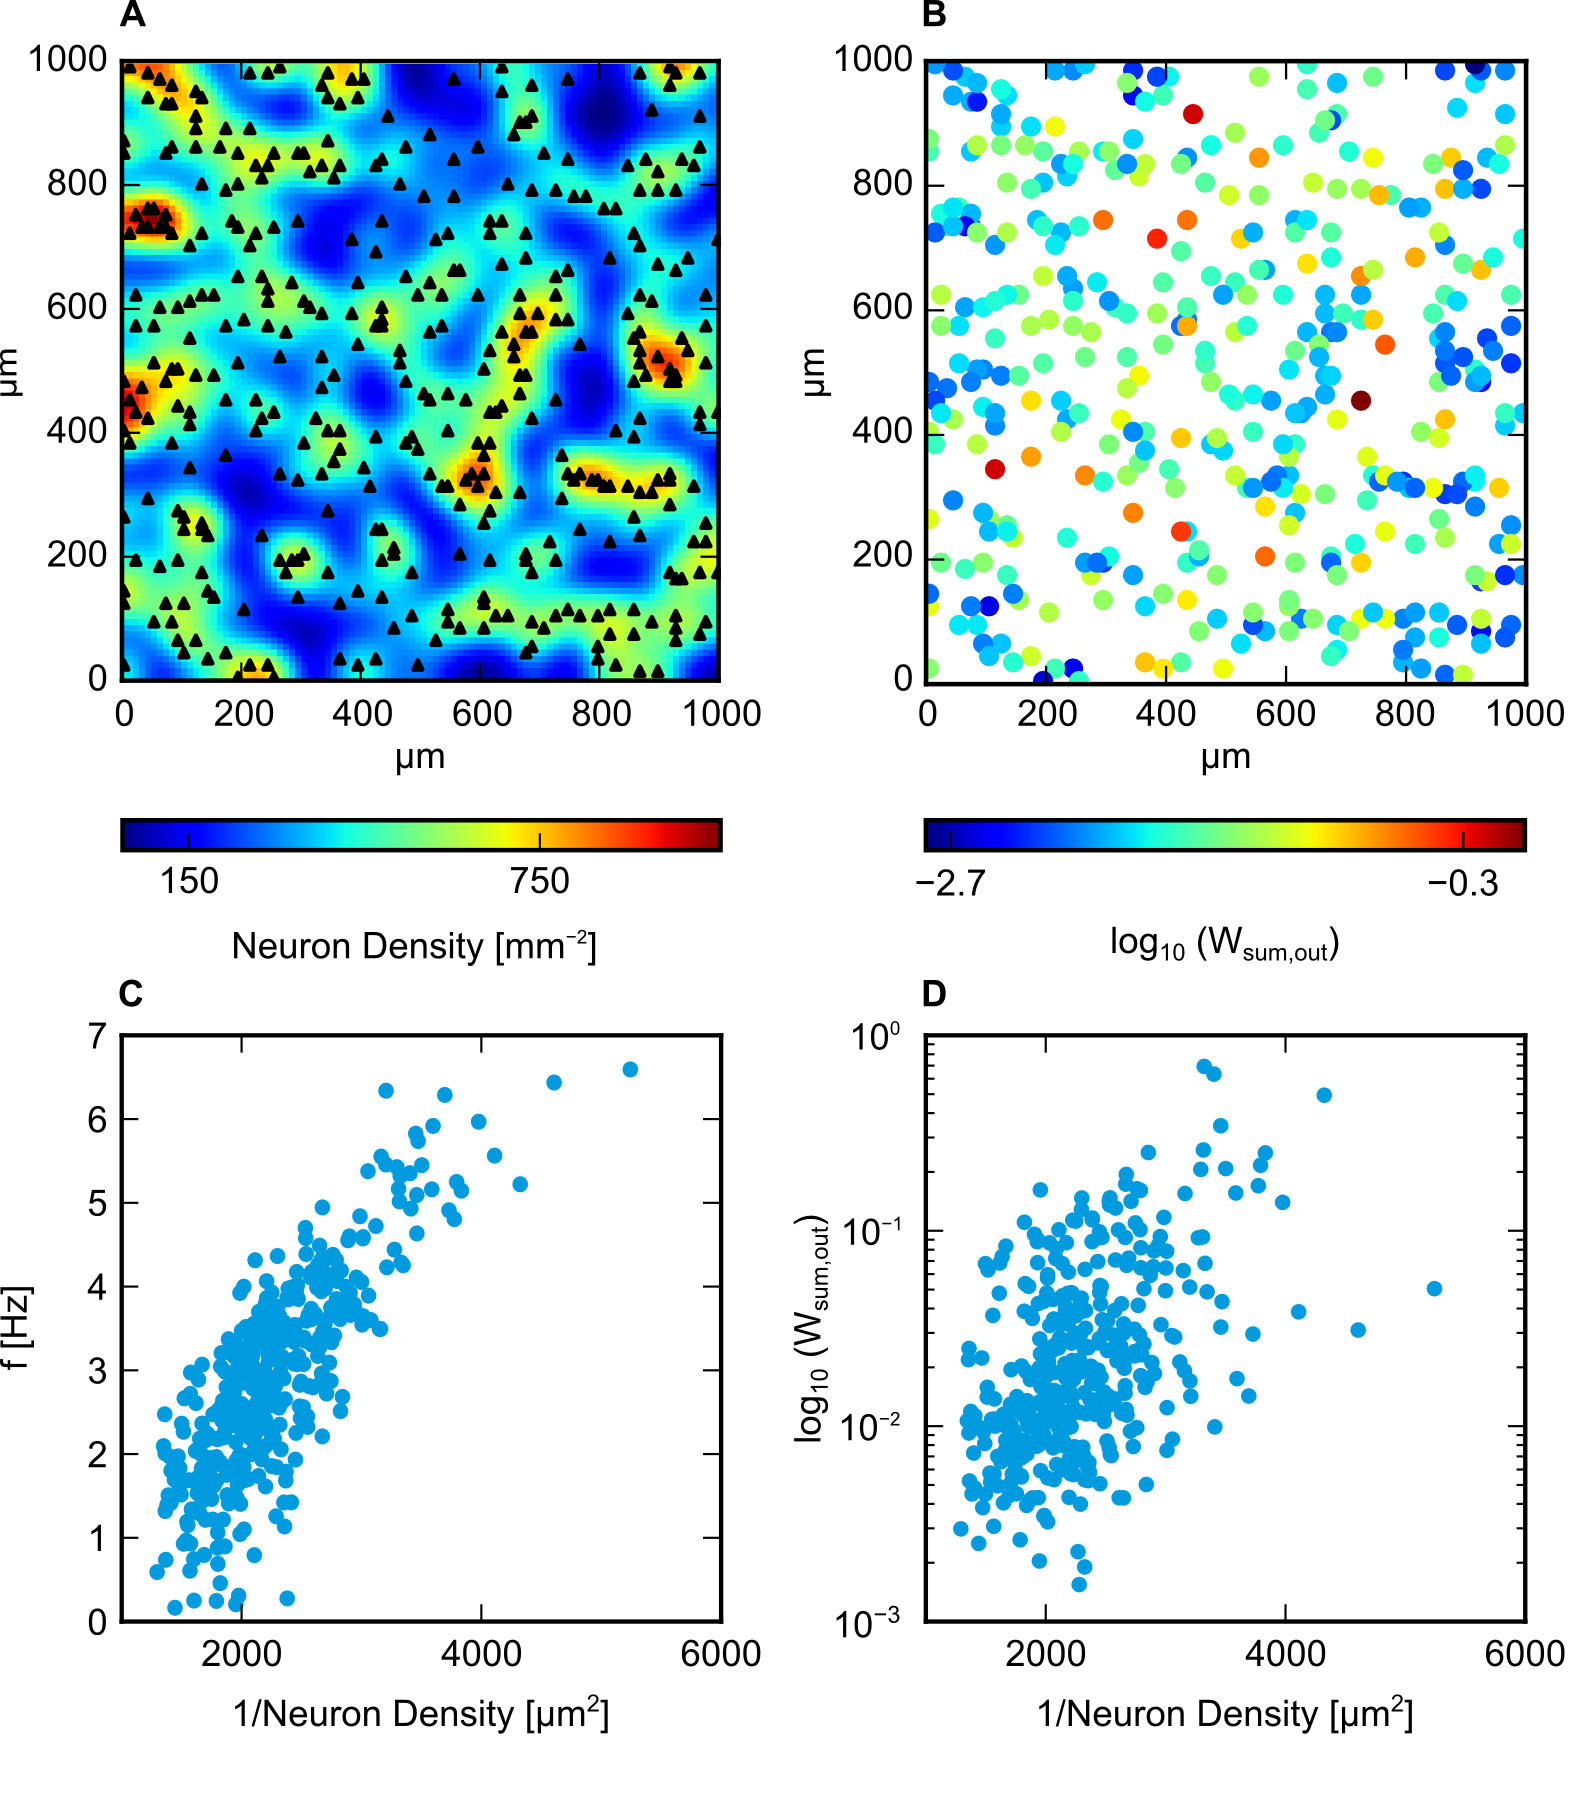
\includegraphics[width=\textwidth]{./figures/scatter_density_out_weights_points_comp_new.png}
\caption{{\bf Mean outgoing excitatory weights vs. reciprocal neuron density.} \textbf{A}: Illustration of excitatory neurons' positions and local neuron density (calculated by convolution with a Gaussian kernel with $\mathrm{\sigma = 50\, \upmu m}$). \textbf{B}: Decadic logarithm of outgoing excitatory weights. Note the spatial correlation between \textbf{A} and \textbf{B} in high/low-density regions. \textbf{C}: Firing rate of excitatory neurons (averaged over $\mathrm{ 1000\,s} \leq t \mathrm{\leq 1500\,s}$) versus reciprocal neuronal density (same estimation method as in A). Coefficient of correlation $\rho = 0.798$. \textbf{D}: Decadic logarithm of mean outgoing excitatory weights versus reciprocal neuronal density. Coefficient of correlation $\rho = 0.513$.}
\label{Inverse_Dens_vs_Sum_Out_Weights}
\end{figure}


\newpage

\section*{Discussion}
The LIF-SORN in combination with diffusive homeostasis presents itself as a \emph{self-organizing} model of cortical activity and plasticity to exhibit core features of neuronal firing statistics as well as synaptic connectivity and dynamics. In order to acquire a deeper understanding of the mechanisms that determine neuronal activity we developed a theory that allowed us to reliably predict the steady-state of firing rates based on the spatial configuration of excitatory neurons. We would like to emphasize that this explanation differs from common approaches of understanding the emergence of heavy-tailed statistics of firing rates in recurrent networks. Theoretical studies on the behavior of recurrent networks are largely based on the assumption that the excitability of neurons is not individually fine-tuned but rather randomly distributed and adjusted globally to achieve a desired mean firing rate. Predictions about the resulting activity are then made based on (potentially simplified) statistical features of recurrent connectivity and/or the specific form of the neuronal transfer function used in the model, see e.g. \cite{Roxin_Firing_Rate_Distribution,Vreeswijk1998,Koulakov_2009}. Our interpretation of our results led us to the conclusion that this approach matches the limiting case of instantaneous diffusion: While Fig.~\ref{Fir_Rate_Dist_Comp}A--D did not reveal many differences between finite-velocity and instantaneous diffusion in terms of overall statistics, the decorrelation shown in Fig.~\ref{Matrix_Predict_Comp}C suggests that increasing the diffusion constant goes along with a transition between a spatially determined configuration of excitatory firing rates and a network topology-determined behavior.

Naturally, this raises the question of biological plausibility. To our knowledge, no experimental study exists that relates measurements of spontaneous activity to local fluctuations of neuronal densities. Interestingly, measurements in the barrel cortex and hippocampus have found that firing rates during exploration or task performance are significantly correlated with those found for spontaneous, baseline activity \cite{OConnor_2010,Mizuseki_2013}. This suggests that the same set of neurons tend to be relatively active or inactive under different stimuli and changing environments. In the light of these observations, one might speculate whether random spatial positioning might at least partially act as a determinant of these individual working points of firing activity. A possible reason for the strong influence of spatial structure in the implemented model could be the fact that cells were modeled as approximate point sources. This allowed for a clear distinction between individual cells, even in close vicinity. While Sweeney et al. argued that the size of the studied tissue is large compared to the size of individual somata (which, apparently, they claim to be the main source of nitric oxide), Philippides et al. reported that NO is often synthesized in a more delocalized way by means of fine fibers originating from the soma \cite{Philippides_2005}. The diameter of these ``production areas" is on the order of $\mathrm{10-100\, \upmu m}$. This suggests that diffusive homeostasis may not act as much as a precise tuner of single neuron activities as found in the computational model. We have shown that the predictions of our analytic approach to obtaining neuronal firing rates are consistent when using more realistic two-dimensional neuronal densities. Interestingly, the predictions for three-dimensional spatial interaction led to a smaller width and skewness of the resulting firing rate distribution. Still, since some amount of heterogeneity could still be observed, we consider it possible that local bunching or isolation of neurons can induce a disposition towards lower/higher long-term firing rates.

The basic assumption that has to be made for this prediction to hold is that NO concentrations are tuned towards a target concentration across neuronal cell bodies. In the theoretical model we used, this was achieved by tuning neuronal excitability by means of a perfect integral control. This might be considered an oversimplification, but does reflect the general idea that NO concentrations must be held within some regime associated with normal neuronal activity. In consequence, it is reasonable to assume that the aforementioned implications of varying neuronal densities still hold at least qualitatively, even if the tuning of NO concentration is not as strict and exact as seen in the theoretical model.

In a recent experimental study, Hengen et al. suggested the existence of ``homeostatic mechanisms that regulate mean firing around cell-autonomous set points" \cite{Hengen_2016}. By means of our analytic predictions regarding homeostatic set points, we have shown that diffusive homeostasis --- in combination with random positioning of cell bodies --- could provide an explanation for these heterogeneous and cell-specific set points of firing rates. However, the study also found that homeostatic regulation is suppressed during sleep. If and how this effect could possibly be incorporated into a model network subject to diffusive homeostasis remains to be clarified.

Despite these considerations regarding the effects of spatial structure onto individual firing rates, our modifications seem to be a plausible way of giving rise to many features of cortical structure and activity. Apart from the previously discussed properties of spiking activity, we have have shown that important features of synaptic topology and plasticity found in earlier research are compatible with diffusive homeostasis. We thereby created a model, which combines the here presented features of cortical structure with the desired statistics of neuronal activity. This was achieved without specific modifications of Hebbian plasticity rules, which have also been proposed as an explanation for log-normally distributed synaptic weights \cite{Koulakov_2009,Gilson_2011,Effenberger_2015}. Sweeney et al. also included synaptic plasticity via STDP into their model, but did not include synaptic normalization, which led to a bimodal distribution of weights, instead of the log-normal like shape obsered in our model \cite{Sweeney_Paper}.

Recent studies have brought up inhibitory-to-excitatory STDP with respect to stabilizing network activity \cite{Vogels_2011,Luz_2012}. Results similar to ours concerning network topology have also been achieved with inhibitory STDP \cite{Effenberger_2015}. In terms of their functional role of stabilizing network activity, it is reasonable to assume that both, diffusive homeostasis and inhibitory STDP, can simultaneously act in a biological system.

In addition, we found that heterogeneity of firing rates led to a much more pronounced separation of mean outgoing weights in our network, which were positively correlated to presynaptic firing rates. This is in line with other theoretical and experimental observations, arguing that a small subset of highly active neurons may serve to form relatively strongly connected and stable subnetworks that can quickly react to momentary changes in the environment, while fine tuned adaptation involves the slower firing majority of cells \cite{Buzsaki_Fir_Rates_2014,Yassin_Subnetworks_2010,Dragoi_2003}. While our observations regarding the influence of diffusive homeostasis onto the network topology can be regarded as an indirect effect, Sweeney and Clopath also investigated the possibility that the diffusion of neurotransmitters could directly affect the dynamics of neural plasticity in a recent theoretical study \cite{Sweeney_2017}, concluding that this promotes stronger synaptic weights between spatially close neurons. It is not clear whether this effect might interfere with our results in a model that combines the effects of diffusive neurotransmitters onto intrinsic, as well as synaptic plasticity: arguing within the scope of our model, two excitatory neurons close to each other will both approximately exhibit half of the firing rate that a single neuron at the same location would have. One could argue that this decrease in activity impedes their probability to form a strong synaptic connection. Future research might therefore involve the implementation of a combined diffusion model to check for these possible interdependencies.

As mentioned previously, models from the SORN family have also proven their capabilities in associative learning and inference tasks \cite{Hartmann_2016}. A logical next step should thus be to test whether the new features presented in this paper can enhance performance in learning, in the sense that the computational and memory resources given by the network size are used more efficiently.

%\section*{Conclusion}
%Our main goal of implementing diffusive homeostasis was to allow a broad distribution of firing rates across the excitatory population of the LIF-SORN, since experimental research has shown this to be a extensively observable phenomenon in the cortex. The implementation of diffusive homeostasis can be regarded as a success with respect to this feature. Furthermore, we did not observe any breakdown of previously studied desirable features of network topology, emerging from the plasticity mechanisms included.

%Our theoretical considerations regarding the steady state of firing activity allowed us to further clarify the actual determinants of the resulting firing rate statistics. It turned out that, depending on the choice of diffusion parameters, a weighted mixture between the distribution of neural inputs and the spatial configuration underlies the resulting statistics of firing rates. The former aspect is in line with common theoretical approaches of explaining firing rate distributions. The latter aspect can be subsumed by the hypothesis that local fluctuations of neuronal density can influence firing rates and shape their overall distribution. This was a rather unconventional idea, and we had to leave the question of biological plausibility unanswered and open to experimental research and possibly more detailed theoretical models of nNOS and its influence onto neural activity.

%The implementation of diffusive homeostasis led to an interesting observation regarding network structure: Due to the broad range of neuronal activity it allowed for the emergence of highly influential subgroups of excitatory neurons. This feature was not present in earlier versions of the LIF-SORN. It can be regarded as another non-random property of cortical structure that was not hard-coded but naturally emerged from the set of basic rules that constitute dynamics and behavior of our network.

%As mentioned previously, the SORN has also proven its capabilities in associative learning and inference tasks \cite{Hartmann_2016}. A logical step should thus be to test whether the new features presented in this paper can enhance performance in learning, in the sense that the computational and memory resources given by the network size are used more efficiently. 

\nolinenumbers

% Either type in your references using
% \begin{thebibliography}{}
% \bibitem{}
% Text
% \end{thebibliography}
%
% or
%
% Compile your BiBTeX database using our plos2015.bst
% style file and paste the contents of your .bbl file
% here. See http://journals.plos.org/plosone/s/latex for 
% step-by-step instructions.
% 
%\newpage
\bibliography{test_base}

%\newpage

\section*{Supporting information}

\paragraph*{S1 Appendix.}
\label{S1_Appendix}
We would like to derive a linear relation between mean firing rate  and the mean rate of NO synthesis. One could naively replace the sum of Dirac functions in \eqref{Ca_dyn} by a continuous inflow ${\rm [Ca^{2+}]}_{\rm spike} r(t)$. This approximation would indeed allow for the correct calculation of a linear relation between mean firing rate and NO production if \eqref{nNOS_dyn} was a linear homogeneous differential equation. The cubic dependence on $Ca^{2+}$ breaks this simplicity. We note the following in order to derive an approximate description: The target firing rate of 3 Hz and the corresponding mean interspike interval of 0.33...s is large compared to the decay constant of calcium, $\tau_{\rm Ca^{2+}} = \mathrm{0.01\,s}$. Consequently, it is very unlikely that one spike event will fall into a region where the calcium concentration, decaying from the instantaneous jump of the previous spike event, is still significantly larger than zero. In fact, calculating the mean concentration of $\rm Ca^{2+}$ before a new spike event over all neurons and all spike events for $\rm 1500\,s$ resulted in a value of $\rm 0.0013$. As such, one can justify the approximation of replacing the exact expression of ${Ca^{2+}}^3(t)$, which is a cubed sum of cut off exponential functions, by a sum of cubed exponentials, because only one term of the sum at a time is significantly larger than zero:
\begin{equation}
\begin{split}
{Ca^{2+}}^3(t) &= \left[ {\rm [Ca^{2+}]}_{\rm spike} \sum_{i} \mathrm{\uptheta} \left( t-t^i_{\rm spike} \right) \exp \left( - \left( t-t^i_{\rm spike} \right) /\tau_{\rm Ca^{2+}} \right) \right]^3 \\
&\approx {{\rm [Ca^{2+}]}_{\rm spike}}^3 \sum_{i} \uptheta \left( t-t^i_{\rm spike} \right) \exp \left( -3 \left( t-t^i_{\rm spike} \right) /\tau_{\rm Ca^{2+}} \right) 
\end{split} \label{cubic_approx_1}			
\end{equation}
with $\uptheta(x)$ being the Heaviside step function. By the same argument
\begin{equation}
\frac{{Ca^{2+}}^3(t)}{{Ca^{2+}}^3(t)+1} \approx \sum_{i} \uptheta \left( t-t^i_{\rm spike} \right) \frac{ \exp \left( -3 \left( t-t^i_{\rm spike} \right) /\tau_{\rm Ca^{2+}} \right) }{\exp \left( -3 \left( t-t^i_{\rm spike} \right) /\tau_{\rm Ca^{2+}} \right) + \frac{1}{{{\rm [Ca^{2+}]}_{\rm spike}}^3}} \; .
\end{equation}
Therefore, the resulting rate of NO synthesis can be decomposed into a sum of time shifted responses onto a single kernel of calcium concentration as a result of a spike. For a spike at $t_{\rm spike}=0$, the solution of \eqref{nNOS_dyn} can be calculated by
\begin{equation}
\begin{split}
nNOS(t) &= \frac{1}{\tau_{\rm nNOS}}\int_{-\infty}^t dt' \exp(-(t-t')/\tau_{\rm nNOS}) \uptheta(t') \frac{\exp(-3t'/\tau_{\rm Ca^{2+}})}{\exp(-3t'/\tau_{\rm Ca^{2+}}) + \frac{1}{{{\rm [Ca^{2+}]}_{\rm spike}}^3}} \\
&= \frac{1}{\tau_{\rm nNOS}}\int_{0}^t dt' \exp(-(t-t')/\tau_{\rm nNOS}) \frac{\exp(-3t'/\tau_{\rm Ca^{2+}})}{\exp(-3t'/\tau_{\rm Ca^{2+}}) + \frac{1}{{{\rm [Ca^{2+}]}_{\rm spike}}^3}}\;.
\end{split}\label{nNOS_single_sol}
\end{equation}



The exact solution of this integral can be expressed in terms of the hyper-geometric function, making it rather impractical for any further analysis. Looking for further simplifications, we noted that $\tau_{\rm nNOS}$ is ten-fold larger than $\tau_{\rm Ca^{2+}}$. This discrepancy in decay times allows for the assumption that the impact of the calcium kernel onto $nNOS$ is practically instantaneous. Consequently, $nNOS(t)$ becomes
\begin{equation}
nNOS(t) = \frac{1}{\tau_{\rm nNOS}} \uptheta(t) \exp(-t/\tau_{\rm nNOS}) \int_{0}^\infty dt' \frac{\exp(-3t'/\tau_{\rm Ca^{2+}})}{\exp(-3t'/\tau_{\rm Ca^{2+}}) + \frac{1}{{{\rm [Ca^{2+}]}_{\rm spike}}^3}}\;.
\label{nNOS_single_sol_approx1}
\end{equation}
In this form, the integral has an easy-to-handle solution, which --- with all spike events now included --- results in
\begin{equation}
nNOS(t) = \frac{{{\rm [Ca^{2+}]}_{\rm spike}}^3 \tau_{\rm Ca^{2+}}\ln(2)}{3\tau_{\rm nNOS}} \sum_i \uptheta(t-t^i_{\rm spike}) \exp(-(t-t^i_{\rm spike})/\tau_{\rm nNOS})\;.
\label{nNOS_single_sol_approx2}
\end{equation}
Fig.~\ref{nNOS_approx_plot} compares the approximation given by \eqref{nNOS_single_sol_approx2} to the full NO production model (equations \eqref{Ca_dyn} and \eqref{nNOS_dyn}). Spikes were drawn from a Poisson process at a rate of 3 Hz. The simplified model fits very well for sufficiently isolated spike events, as predicted. One can observe a slightly smaller but acceptable agreement for the rare event of two subsequent spikes appearing very close to each other, as seen in Fig.~\ref{nNOS_approx_plot} at approximately 4 seconds.

\begin{figure}[h]
%%% ca_nnos_test.py
\begin{center}
%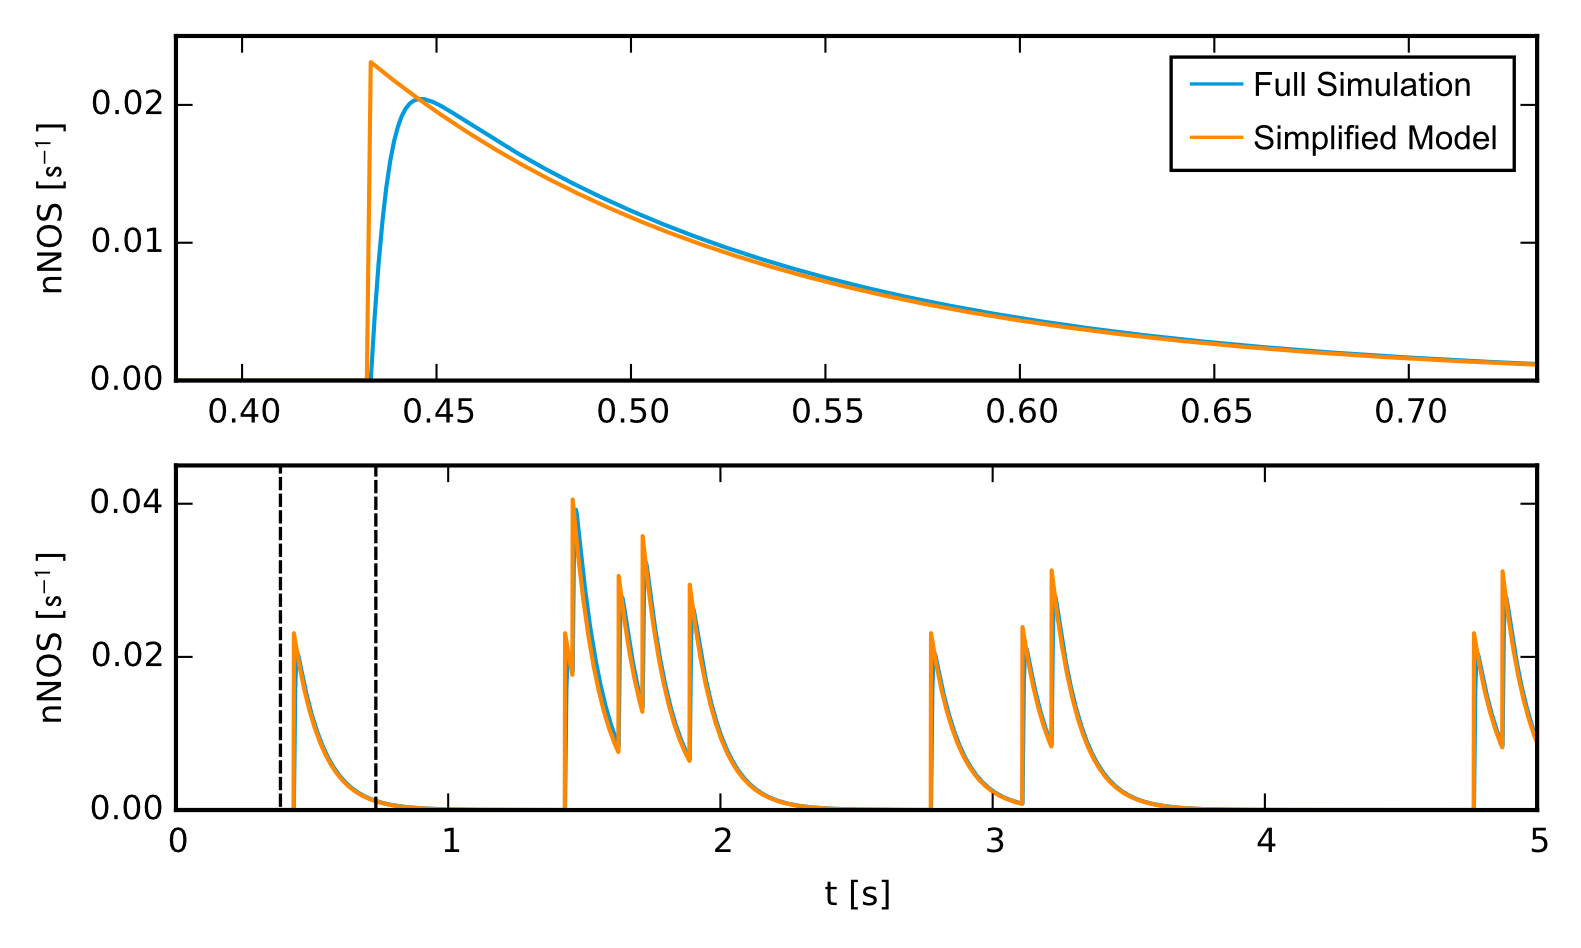
\includegraphics[width=\textwidth]{./figures/nNOS_approx.png}
\end{center}
\caption{{\bf nNOS under Poisson spiking.} Time course of nNOS(t) with Poisson spiking at 3 Hz. The full simulation (blue, see equations \eqref{Ca_dyn},\eqref{nNOS_dyn}) is well fitted by the simplified model (red, see \eqref{nNOS_single_sol_approx2}). Top axis is a closeup of the first spike event.}
\label{nNOS_approx_plot}
\end{figure}

Thus, on average, the sum in \eqref{nNOS_single_sol_approx2} simply reduces to the mean rate $\langle r \rangle$:
\begin{equation}
\langle nNOS \rangle = \frac{{{\rm [Ca^{2+}]}_{\rm spike}}^3 \tau_{\rm Ca^{2+}}\ln(2)}{3\tau_{\rm nNOS}} \langle r \rangle \; .
\label{nNOS_single_sol_approx3}
\end{equation}

\end{document}

